\documentclass[a4paper,12pt]{article}
%\documentclass[11pt,twoside,a4paper]{book}
\usepackage{float}
\usepackage{graphicx} %pacote pra colocar imagem
\graphicspath{ {images/} }
\usepackage[utf8]{inputenc}
\usepackage[brazil]{babel}
% \usepackage{cite}

 \usepackage{setspace}                   % espaçamento flexível
 \usepackage{indentfirst}                % indentação do primeiro parágrafo
 \usepackage[fixlanguage]{babelbib}
 \usepackage[font=small,format=plain,labelfont=bf,up,textfont=it,up]{caption}
 \usepackage[usenames,svgnames,dvipsnames]{xcolor}
%  \usepackage[a4paper,top=2.54cm,bottom=2.0cm,left=2.0cm,right=2.54cm]{geometry} % margens
 \usepackage{amsmath,amssymb,exscale}

%  \usepackage[pdftex]{hyperref}
 \usepackage[pdftex,plainpages=false,pdfpagelabels,pagebackref,colorlinks=true,citecolor=DarkGreen,linkcolor=NavyBlue,urlcolor=DarkRed,filecolor=green,bookmarksopen=true]{hyperref} % links coloridos
 \usepackage[all]{hypcap}                    % soluciona o problema com o hyperref e capitulos
 \usepackage[round,sort,nonamebreak]{natbib} % citação bibliográfica textual(plainnat-ime.bst)
 \bibpunct{[}{]}{;}{n}{\hspace{-0.7ex},}{,} % estilo de citação. Veja alguns exemplos em http://merkel.zoneo.net/Latex/natbib.php

 \usepackage{pdfpages}

%  \fontsize{60}{62}\usefont{OT1}{cmr}{m}{n}{\selectfont}

 \usepackage{listings}

\usepackage{color}
\definecolor{editorGray}{rgb}{0.95, 0.95, 0.95}
\definecolor{editorOcher}{rgb}{1, 0.5, 0} % #FF7F00 -> rgb(239, 169, 0)
\definecolor{editorGreen}{rgb}{0, 0.5, 0} % #007C00 -> rgb(0, 124, 0)
\usepackage{upquote}
\usepackage{listings}
\lstdefinelanguage{JavaScript}{
  morekeywords={typeof, new, true, false, catch, function, return, null, catch, switch, var, if, in, while, do, else, case, break},
  morecomment=[s]{/*}{*/},
  morecomment=[l]//,
  morestring=[b]",
  morestring=[b]'
}

\lstdefinelanguage{HTML5}{
        language=html,
        sensitive=true,
        alsoletter={<>=-},
        otherkeywords={
        % HTML tags
        <html>, <head>, <title>, </title>, <meta, />, </head>, <body>,
        <canvas, \/canvas>, <script>, </script>, </body>, </html>, <!, html>, <style>, </style>, ><
        },
        ndkeywords={
        % General
        =,
        % HTML attributes
        charset=, id=, width=, height=,
        % CSS properties
        border:, transform:, -moz-transform:, transition-duration:, transition-property:, transition-timing-function:
        },
        morecomment=[s]{<!--}{-->},
        tag=[s]
}

\lstset{%
    % Basic design
    backgroundcolor=\color{editorGray},
    basicstyle={\scriptsize\ttfamily},
    frame=l,
    % Line numbers
    xleftmargin={0.75cm},
    numbers=left,
    stepnumber=1,
    firstnumber=1,
    numberfirstline=true,
    % Code design
    keywordstyle=\color{blue}\bfseries,
    commentstyle=\color{darkgray}\ttfamily,
    ndkeywordstyle=\color{editorGreen}\bfseries,
    stringstyle=\color{editorOcher},
    % Code
    language=HTML5,
    alsolanguage=JavaScript,
    alsodigit={.:;},
    tabsize=2,
    showtabs=false,
    showspaces=false,
    showstringspaces=false,
    extendedchars=true,
    breaklines=true,
    % Support for German umlauts
    literate=%
    {Ö}{{\"O}}1
    {Ä}{{\"A}}1
    {Ü}{{\"U}}1
    {ß}{{\ss}}1
    {ü}{{\"u}}1
    {ä}{{\"a}}1
    {ö}{{\"o}}1
}

\newcommand{\code}[1]{\lstinline[mathescape=true, columns=fixed, basicstyle={\small\ttfamily}]{#1}}


 \usepackage{fancyvrb}

\title{Trabalho de Conclusão de Curso}
\author{Guilherme Freire Silva}
\date{\today}

% ---------------------------------------------------------------------------- %
% INFORMAÇÕES

\pdfinfo{%
  /Title    (Comunicação cliente-servidor bilateral de baixa latência aplicado a Android)
  /Author   (Guilherme Freire Silva)
  /Subject  (Trabalho de Conclusão de Curso)
  /Keywords (TCC, Socket, Android)
}






\begin{document}
\pagenumbering{gobble}
% ---------------------------------------------------------------------------- %
% CAPA
% Nota: O título para as dissertações/teses do IME-USP devem caber em um
% orifício de 10,7cm de largura x 6,0cm de altura que há na capa fornecida pela SPG.

\thispagestyle{empty}
\begin{center}
    \vspace*{2.3cm}
    \textbf{\Large{Comunicação cliente-servidor bilateral de baixa latência aplicado a Android}}\\


    \vspace*{1.2cm}
    \Large{
        Guilherme Freire Silva
    }
    \vskip 2cm
    \textsc{
     Trabalho de Conclusão de Curso \\[-0.25cm]
    Instituto de Matemática e Estatística\\[-0.25cm]
    da\\[-0.25cm]
    Universidade de São Paulo\\[-0.25cm]%}
    }

    \vskip 2.5cm
    Orientador: Prof. Dr. Marco Dimas Gubitoso

    \vskip 3.5cm
    \normalsize{São Paulo, 2016}
\end{center}

\newpage

\newpage
\section{Resumo}

Desenvolvimento de um ambiente Web com três tipos de elementos diferentes. Desenvolvimento de um aplicativo mobile em Apache Cordova. Desenvolvimento de uma página Web 3D com THREE.JS. Criação de um servidor utilizando Node.js e Express.js. Comunicação entre os três elementos utilizando o protocolo WebSocket com o framework Socket.io.

\textbf{Palavras-chave}: Socket.io, Node.js, Express.js, THREE.JS, Apache Cordova.


\newpage
\tableofcontents

\newpage
% \pagenumbering{arabic}     % começamos a numerar

\renewcommand{\arraystretch}{1.2}











% \newpage
% \section{Abstract}

% Web environment development with three distinct types of elements. Mobile development with Apache Cordova. 3D Web development with THREE.JS. Server-side aplication with Node.js and Express.js. Communication between these three elements with WebSocket protocol and Socket.io framework.

% \textbf{keywords}: Socket.io, Node.js, Express.js, THREE.JS, Apache Cordova.


\newpage
\section{Introdução}

O Projeto para o Trabalho de Formatura Supervisionado apresentado nessa monografia tem como objetivo explorar tecnologias e ferramentas presentes no cotidiano de forma inovadora.

Uma das tecnologias exploradas foi a de smartphones. Eles são dispositivos muito sofisticados, possuem muitas funcionalidades, como acesso à internet, alto poder de processamento, tela de toque, diversos sensores, Bluetooth, WiFi, dentre outros.

Além de diversas funcionalidades, a capacidade de desenvolvimento para essa plataforma é muito grande, os principais Sistemas Operacionais (Android e iOS) permitem essa liberdade de desenvolvimento em sua plataforma, oferecendo o suporte necessário para tal.

Existe também uma gama de ferramentas para o desenvolvimento mobile, com as mais diversas metodologias, além de uma ativa comunidade online para dar suporte e documentar erros e boas práticas.

Atualmente, a maior parte dos aplicativos para smartphones usam a conectividade com a internet para recolher dados e exibí-los, de uma forma ou de outra, para o usuário. Alguns exemplos dessa estrutura são:

\begin{itemize}
    \item Em um aplicativo de notícias, o sistema recebe do servidor uma lista de notícias. O usuário pode ter um conjunto de preferências enviadas ao servidor para receber um conteúdo mais específico.

    \item Em um aplicativo de localização, o sistema recebe dados do GPS e envia ao servidor, para receber o mapa dos arredores da posição enviada.

    \item Em jogos, talvez parte do conteúdo (como sons e imagens) não esteja no baixado ainda, então ele faz o download quando o jogador faz certas ações. O jogo também pode enviar o progresso ao servidor como backup, para ser restaurado quando necessário.
\end{itemize}

Ao analisar esse comportamento, fica claro como o usuário só interage com seu dispositivo, toda a comunicação externa é um resultado disso. Na maioria dos casos, o usuário não tem ativamente o propósito de alterar coisas fora do espaço de seu smartphone.

\begin{itemize}

    \item Um contra-exemplo dessa estrutura é o aplicativo Unified Remote \footnote{https://www.unifiedremote.com/, acessado em 05/02/17.}. Ele oferece um controle remoto para o seu computador. Para funcionar, é necessário instalar um software no computador a ser controlado e tanto ele, como o smartphone devem estar conectados à mesma rede WiFi. Então, com o smartphone, é possível controlar o cursor, o volume do som, teclado, dentre outros.

\end{itemize}

Esse fato impulsionou esse Projeto em criar um ecossistema composto por um aplicativo e um servidor. O diferencial é que o aplicativo não é o único produto com o qual o usuário está interagindo de forma direta, mas sim o servidor também, de forma tangível.

A ideia é que o usuário faça ações no aplicativo, e veja o resultado dessas ações diretamente no servidor. O smartphone deixa de ser o produto final, e se torna somente uma forma de input de dados para um sistema maior.

Um resultado desejado é que ações originadas no servidor também surtam efeito no aplicativo, para mostrar que é possível uma comunicação bilateral sem hierarquias entre os dois lados desse sistema.

Outro resultado desejado é que seja possível conectar mais de um smartphone com esse servidor, para que ambos possam interagir com ele e talvez até entre si.


Existem alguns exemplos de aplicativos e projetos que possuem uma estrutura similar:

\begin{itemize}

    % TODO https://vimeo.com/48150517
    % TODO http://www.webdigi.co.uk/fun/space/
    \item Na palestra de Roshan Abraham entitulada “Using your iPhone as a game controller with NodeJS, HTML5" é apresentado um trabalho cuja estrutura é quase idêntica ao Projeto desenvolvido.

    No trabalho, existe um servidor que lança uma página Web com um \emph{QR Code} no computador do usuário. Quando um dispositivo que roda o Sistema Operacional iOS (iPhone ou iPad) lê esse código, ele executa uma página Web que envia dados do acelerômetro ao servidor. O servidor por sua vez, ao receber essa conexão, envia ao navegador no computador um jogo de “\emph{Space Invaders}". Nesse jogo, a nave é controlada pelas leituras do acelerômetro; ou seja, ao inclinar o dispositivo para um lado, ela vai acompanhar esse movimento.

    A diferença entre esse trabalho e o Projeto apresentado aqui é que ele se limita à iOS e utiliza uma página Web no dispositivo, ao invés de um aplicativo dedicado. Por utilizar o browser do dispositivo como aplicativo, ele é limitado aos recursos e funcionalidades que esse browser tem acesso.

    % www.airconsole.com
    \item AirConsole - Uma plataforma de jogos online, na qual cada jogador usa seu smartphone como controle e a tela do computador exibe o jogo. Ele funciona de maneira similar ao exemplo de cima, porém é um produto finalizado, muito mais robusto.

    Essa plataforma oferece duas maneiras de usar o smartphone, é possível se conectar através de um browser (como no exemplo acima) ou usar um aplicativo (como esse Projeto propõe). Para se conectar, o computador exibe um código e o jogador o insere no smartphone. É possível conectar multiplos jogadores em uma única sessão, para que o jogo seja \emph{multiplayer}. Cada jogo também apresenta um layout diferente de controle para o smartphone.

    A plataforma também disponibiliza um API \footnote{\emph{Application program interface}} para o desenvolvimento, então é possível usá-la para criar jogos de forma livre.

    Todas as funcionalidades dessa plataforma são desejáveis para este Projeto, ele é o que mais se aproxima do ideal. Porém, essa plataforma é somente para jogos e usa servidores próprios, deixando o processamente no lado do servidor fechado aos desenvolvedores. O projeto foi pensado para satisfazer uma gama maior de necessidades, não somente de jogos, e dar a liberdade ao desenvolvedor de alterar o código do servidor, para adequar melhor suas necessidades.

\end{itemize}





\newpage
\subsection{Objetivos}

\begin{itemize}
    \item Estudar a comunicação servidor x cliente mobile.

    \item Construir uma estrutura eficiente de comunicação.

    \item Validar o uso da estrutura através de uma página Web e um Aplicativo.


    % \item Desenvolver um aplicativo para smartphones.

    % \item Criar um servidor.

    % \item Construir uma comunicação entre ambos.

    % \item Encontrar uma forma eficiente de comunicação.

    % \item Desenvolver uma página Web como Caso de Uso.
\end{itemize}



Em suma, o objetivo desse Projeto é criar um sistema composto por um aplicativo e um servidor que interagem entre si, proporcionando ao usuário uma experiência mais completa do que a que os aplicativos de hoje oferecem.

Como o desenvolvimento desse sistema é bastante extenso, o foco será somente na criação dele como um arcabouço para o desenvolvimento de aplicações maiores. Não haverá uma aplicação que utilize seu pontencial máximo, somente uma que valide os objetivos propostos.

% De forma concreta, ao final do desenvolvimento é esperado que exista esse ecossistema online, com o servidor e os dois clientes, de Android e Web. O aplicativo Android deve gerar dados e os enviar ao servidor, além de receber dele. A página Web deve executar um programa interativo que recebe dados do servidor a qualquer momento para alterar sua execução. E, por fim, o servidor precisa funcionar como intermediador dos dados, enviando e recebendo dados de cada cliente quando for necessário.

% TODO Qual a diferença entre web-page + server e webservice?






\newpage
\section{Fundamentos}

Esta seção explica conceitos que são utilizados no Projeto, ou que ajudam a entender a tecnologia usada e as decisões tomadas.

\subsection{Estrutura e funcionamento de páginas Web}

Uma página Web (\emph{webpage}) é o produto final gerado por arquivos HTML, CSS, JavaScript, imagens e outros recursos (\emph{resources}). A webpage é interpretada por um \emph{Web Browser}, que interage com o usuário, tanto exibindo informações, quanto recebendo \emph{inputs}. Cada um desses elementos citados se comporta da seguinte forma:

\begin{itemize}
    \item HTML \emph{Hyper Text Markup Language} - É a linguagem que descreve como uma webpage deve ser formatada. Para isso, ela funciona através de um conjunto de \emph{tags}, cada uma com uma função diferente. Elas definem conteúdo (o texto propriamente dito), formatação (alteração de tamanho, cor, fonte) inserção de recursos externos (imagens, áudios, vídeos, caixas de inserção de texto), fluxo entre páginas (\emph{hiperlinks}, redirecionamentos, auto rolagem da página, definição de segmentos de conteúdo) execução de código lógico (inserção de scripts para processamento de dados), dentre outros. O principal arquivo de uma webpage é um HTML, que dita sua estrutura, formatação e conteúdo.

    \item CSS (\emph{Cascading Style Sheets}) - É um arquivo de suporte para HTML cujo propósito é definir estilos de formatação. Ele centraliza o processo de formatação de estilos e dá opções mais refinadas de customização. Não é necessário, porém é muito importante na criação de estilos mais complexos, para webpages mais robustas e profissionais.

    \item JavaScript - É a linguagem de programação de scripts executados em HTML. É o responsável pela parte lógica do funcionamento de uma webpage, executando código dentro dela, com dados externos ou do usuário. Usando scripts é possível criar timers, contadores, atualizar informações exibidas, carregar conteúdo dinamicamente, renderizar outros tipos de objetos na tela, entre outros. Uma webpage que usa scripts de forma inteligente é mais interativa e possui muito mais recursos.

    \item Web Browser - Um \emph{browser}, ou navegador, é o programa que exibe webpages. Para exibir uma página que o usuário pede, ele se conecta ao servidor, a recebe e interpreta e então a exibe na tela.

    \item Servidor Web - Um servidor web é um processo em execução possui webpages e seus recursos (CSS, JavaScript, imagens). Ele possui um endereço IP para ser localizado por browsers na internet e, após uma conexão ser feita, ele envia as páginas requisitadas ao browser. Os servidores são capazes de lidar com múltiplas conexões.

\end{itemize}



\subsection{Comunicação Web}

Para que conexões através da internet sejam possíveis, como uma conexão entre um browser e um servidor por exemplo, uma arquitetura de rede adequada é necessária. A arquitetura mais comum para este uso é o modelo cliente-servidor.

Neste modelo, existem dois tipos de programas sendo executados:

\begin{itemize}
    \item O Cliente é o programa que precisa receber dados da internet. Browsers, por exemplo, para poder exibir uma página, precisam requisitá-la de algum lugar. O usuário insere o endereço do site que deseja, e então o browser pede a esse endereço a página que gostaria.

    Nesse pedido, ele também envia outros tipos de informações, como seu próprio endereço, alguns dados do usuário, detalhes do que está requisitando, dados e \emph{tokens} de segurança, entre outros.

    Ele recebe como resposta uma página e todos os recursos necessários para que ela seja visualizada corretamente (é possível também receber mensagens de erro caso ocorra qualquer falha, como erros nos dados enviados ou problemas de conexão). Essa página pode trazer dados que permitem o acesso à outra página, gerando um fluxo de telas.

    \item O Servidor é o programa que opera do outro lado da conexão. Ele possui endereço e dados de uma webpage (os arquivos HTML, CSS, JavaScript e outros recursos) e, uma vez em execução, ele aguarda pedidos vindos de clientes.

    Ao receber uma requisição, ele verifica os dados do cliente, da requisição, de segurança, dentre outros. Se tudo estiver correto e ele possuir o que é pedido, é enviada uma resposta contendo esses arquivos. Caso contrário, a resposta contém somente uma mensagem de erro, para que o cliente possa corrigir e fazer uma nova requisição.

    Por fim, um servidor tem a capacidade de receber requisições de vários cliente ao mesmo tempo. A cada requisição, ele executa seu processamento, envia a resposta adequada e atende o seguinte.
\end{itemize}

É importante explicitar que esse modelo não serve somente para transportar páginas Web pela internet, ele é mais abstrato, transporta serviços. Servidores podem armazenar bancos de dados e clientes podem requisitar buscas (\emph{queries}) a eles; o servidor pode somente armazenar arquivos do usuário (em serviços de backup em Nuvem, como o Dropbox\footnote{dropbox.com}) e o cliente requisita o download ou upload de arquivos.

Em resumo, no modelo cliente-servidor, há dois tipos de processo sendo executados, o cliente e o servidor. O cliente necessita de um serviço que o servidor oferece. Ele então gera uma requisição e a envia ao servidor. Se tudo ocorrer bem, o servidor envia uma resposta contendo os dados que o cliente necessita. A conexão é encerrada e o servidor volta ao estado de espera por outras requisições.

\subsection{Protocolo HTTP}

O protocolo HTTP (\emph{Hypertext Transfer Protocol}) é o principal protocolo do modelo cliente-servidor, lidando com a transferência de dados via Web.

Este protocolo está implementado tanto no cliente, como no servidor. Ele se encarrega de abrir a conexão entre ambos; de formar as mensagens a serem enviadas, como requisições e respostas, e fazer a transferência desses dados, sejam arquivos HTML, JavaScript, imagens, ou qualquer outro recurso.

Ele é um protocolo sem estado, os processos não salvam informações sobre cada conexão. Cada mensagem enviada contém todo o contexto necessário para ser compreendida e respondida.

Alguns conceitos importantes sobre comunicação:

\begin{itemize}
    \item Latência. É o tempo entre uma mensagem ser enviada por um sistema e ser recebida pelo outro. Pelas propriedades físicas de uma conexão (distância real entre o cliente e o servidor, velocidade de impulsos elétricos) esse tempo é um fator real e que deve ser levado em consideração durante o desenvolvimento de um sistema online.

    A forma mais básica e direta de se calcular a latência com um servidor é fazer um \emph{ping}. Essa técnica consiste fazer uma requisição vazia ao servidor pedindo resposta vazia de volta e calcular o tempo entre o momento que uma mensagem foi enviada e outra foi recebida.

    \item HTTP é um protocolo sem estado. Os processos que participam de conexão não guardam dados sobre ela. Quando uma mensagem é enviada, todos os dados necessários para sua compreensão são enviados juntos.

    Uma conexão nesse contexto não é algo longo, dura somente o tempo entre o cliente mandar a requisição e receber a resposta.

    \item Cabeçalho de uma mensagem. Quando uma mensagem é formada, ela não pode ter somente seu conteúdo, é necessário que haja outras informações junto, para que possa ser compreendida. O cabeçalho pode conter um identificador do usuário, tipo do conteúdo da mensagem, dados de conexão e segurança, entre outros. Essas informações são necessárias, porém aumentam o tamanho da mensagem final que será enviada.

    \item Um servidor HTTP não possui autonomia para enviar dados a um cliente espontaneamente, ele só pode enviar quando a mensagem é uma resposta a uma requisição do cliente.
\end{itemize}


\subsection{Sockets}

Em contraponto com os tópicos anteriores, sockets são elementos da comunicação Web bastante concretos. Dentre os componentes presentes na estrutura que implementa um protocolo de comunicação, como HTTP ou P2P, o socket é aquele cujo propósito é efetivamente mandar e receber informação. Ele é a porta de entrada e saída de dados de um processo que se comunica com outros através da internet.

Como eles são componentes internos, cada protocolo os utiliza de uma certa maneira. No modelo cliente-servidor por exemplo, o socket do servidor tem o poder de enviar informações a um cliente a qualquer momento, mas o protocolo só permite o envio de respostas a uma requisição, nunca um envio espontâneo.

Cada socket possui um endereço único para ser localizado na Web, a união do endereço de IP e uma Porta, definida pelo processo. Toda conexão Web é concretamente definida através do par de sockets, um de cada processo.






\newpage
\section{Modelo e definição de funcionamento}


Uma vez que a ideia geral do Projeto está fechada, é necessário definir como a estrutura vai funcionar exatamente e encontrar um modelo que satisfaça as necessidades definidas.

No âmbito geral temos dois softwares a serem desenvolvidos, um aplicativo para smartphones e um servidor. Eles devem estar sendo executados simultaneamente e cada um deve interferir com o outro diretamente. O foco é ter um produto que mostre que essa arquitetura funciona de forma satisfatória.

Os requerimentos do servidor:

\begin{itemize}

    \item Ser capaz de receber conexões e dados vindos de smartphones.

    \item Enviar dados para esses smartphones que foram conectados à rede.

    \item Exibir um feedback visual de sua execução.

    \item Permitir que os dados que recebe do smartphone alterem sua execução de forma concreta.

\end{itemize}

Os requerimentos do aplicativo:

\begin{itemize}

    \item Conectar-se a um servidor específico.

    \item Conseguir enviar dados a esse servidor a qualquer momento.

    \item Receber dados desse servidor a qualquer momento.

    \item Ter uma interface que permita inputs variados.

\end{itemize}

Para começar a estruturação, o primeiro ponto a ser aprofundado é a visualização que se espera do processamento do servidor.

Um servidor possui um código estritamente lógico, não é possível fazer uma aplicação direta nele, precisa haver algo para intermediar essa interface. A maneira mais natural para que isso ocorra é fazer ele gerar uma webpage que recebe seus dados e faz um processamento próprio.

Essa webpage é uma aplicação que será executada em um cliente e reduz a carga de dados a ser processada pelo servidor\footnote{É uma boa prática de desenvolvimento deixar o mínimo de processamento possível à cargo do servidor, pois ele pode estar lidando com uma quantidade muito grande de dados vindos de outros clientes.}. Essa situação torna necessário novos requerimentos a serem levados em consideração.

Os requerimentos para essa nova webpage:

\begin{itemize}

    \item Receber dados do servidor sempre que eles forem atualizados.

    \item Executar uma aplicação que use esses dados de forma concreta.

\end{itemize}

A estrutura fica mais clara com esses três elementos trabalhando juntos, o aplicativo, o servidor e a webpage. O aplicativo vai se conectar ao servidor e iniciar sua troca de dados enquanto é executado. O servidor faz um processamento leve desses dados e os emite à webpage, executada em outro cliente. A webpage, enquanto executa uma aplicação, recebe, processa e incorpora esses dados a si, alterando os resultados de sua execução.

O próximo passo é analisar e definir concretamente cada componente deste ecossistema:





\newpage
\subsection{Comunicação}

A comunicação entre o servidor e os clientes é o ponto mais importante deste sistema. Idealmente, ele deve satisfazer os seguintes requerimentos:

\begin{itemize}

    \item \textbf{Baixa latência.} Comandos emitidos pelo aplicativo precisam ser executados pela webpage com o menor tempo de delay possível, caso contrário a experiência de uso pode ser danificada. Existem casos de aplicativos nos quais latência alta não é um problema, mas existem outros que necessitam dessa resposta imediata (como jogos, por exemplo).

    \item \textbf{Baixo \emph{overhead} de mensagens.} É necessário que o tamanho de mensagens enviadas seja o menor possível. O principal fator negativo desse requerimento é o cabeçalho dessas mensagens.

    No caso de mensagem com muito conteúdo, ele faz pouca diferença para o tamanho total. Para mensagens pequenas, como um texto ou um conjunto de valores, o cabeçalho é um aumento significativo no tamanho total, podendo ser até maior do que o próprio conteúdo.

    Para um fluxo de mensagens alto, um cabeçalho proporcionalmente grande consumi muita banda da conexão e recursos, tanto do servidor como dos clientes. É necessário então que possua a menor quantidade de informações desnecessárias.

    \item \textbf{Comunicação bilateral.} Informações podem se originar de qualquer um dos clientes ou do servidor, então é necessário que o processo em questão possa enviar dados a qualquer momento. Um cliente precisar consultar o servidor a intervalos regulares de tempo para saber se há dados novos inviabiliza o sistema proposto.

    \item \textbf{Permitir multiplas conexões simultâneas.} Deve ser possível para o servidor aceitar a conexão de múltiplos smartphones durante sua execução, e gerenciar os dados de cada um. Não é um requerimento, mas aumenta o grau de liberdade do sistema.

\end{itemize}

O modelo cliente-servidor é ideal para esses requerimentos, porém é necessário levar alguns pontos em consideração. O aplicativo e a webpage precisam se comunicar com o servidor da melhor forma possível e o protocolo de comunicação é o fator que mais pode limitar as possibilidades previstas.

As limitações do protocolo HTTP não permitem que ele seja usado, então é adotado o uso do protocolo WebSocket, utilizando Socket.io, um Framework de JavaScript.


\subsubsection{Protocolo WebSocket}

WebSocket é um protocolo que permite a comunicação bilateral entre cliente e servidor. Para o protocolo, não existe essa diferenciação entre os dois, o cliente e o servidor são apenas dois processos conectados. A comunicação é dada por envio de mensagens e ocorrência de eventos. Esses processos podem enviar mensagens a qualquer momento e estão ouvindo um ao outro.

A estrutura da mensagem em WebSocket é mínima. O corpo da mensagem, os dados a serem enviados, só possui dois formatos, texto ou binário. O cabeçalho contém um identificador de tipo do formato, que tem um campo para o tamanho da mensagem e nada mais. A mensagem completa é composta pelo conteúdo e seu tamanho. Como a conexão não muda em momento algum, todas as informações contidas no cabeçalho de requisição e resposta HTTP são invariantes e, portanto, não precisam ser reenviadas, sendo armazenadas no processo.

Um dos processos conectados, em um momento arbitrário, envia uma mensagem ao outro, talvez porque dados tenham sido atualizados ou o usuário tenha feito alguma ação em específico. Uma vez que a mensagem é enviada, esse processo volta ao que estava fazendo, sem a necessidade de esperar alguma resposta do outro processo. Esse comportamento é chamado de assíncrono, pois um lado não age em sincronia com o outro.

O outro processo recebe a nova mensagem através de um evento. Quando esse evento acontece, ele executa um comportamento específico (\emph{callback}) com os dados recebidos, como alteração de informações exibidas ou um cálculo com os valores novos. Por isso é dito que WebSocket é orientado a eventos.


\subsubsection{Socket.io}

Socket.io é a API de WebSocket para JavaScript a ser utilizada. Além da implementação básica do protocolo, ele também adiciona outras funcionalidades importantes para o desenvolvimento de uma aplicação robusta. As funcionalidades mais interessantes para o sistema são:

\begin{itemize}

\item \textbf{A possibilidade de conectar múltiplos sockets em uma mesma porta}. Utilizando WebSockets, cada socket precisa de uma porta exclusiva para fazer a conexão.

\item \textbf{Criação arbritrária de eventos}. Com WebSocket, o desenvolvedor fica preso a quatro eventos pré definidos: \emph{onopen}, \emph{onclose}, \emph{onmessage} e \emph{onerror}.

Essa criação de eventos funciona da seguinte forma: o processo emissor manda a mensagem e o nome do evento que está sendo enviado. O processo receptor define o evento que vai ouvir e a subrotina que vai ser executada na ocorrência desse evento. Se o evento lançado for ouvido pelo receptor, o \emph{callback} é chamado.
\end{itemize}

Socket.io será utilizado para a comunicação em todos os componentes.% Todos os processos escutam e enviam eventos entre si, e o servidor permite a conexão de múltiplos clientes.



\newpage
\subsection{Aplicativo para Smartphone}

O aplicativo deve seguir a proposta de servir como base para o desenvolvimento de aplicativos maiores. Sobre seu funcionamento nesse projeto, ele vai permitir as seguintes ações:

\begin{itemize}

  \item \textbf{Se conectar e desconectar de um servidor}. Vai existir um campo para se inserir o IP e Porta do servidor, e um botão de “conectar". Ao inserir o endereço do servidor e clicar no botão, a conexão será feita. Outro clique fará com que a conexão seja encerrada.

  \item \textbf{Capturar leituras do acelerômetro\footnote{Sensor que mede a aceleração do movimento do dispositivo.}}. O aplicativo conseguirá obter informações de aceleração espacial do smartphone.

  \item \textbf{Emitir eventos pontuais ao servidor}. A interface apresentará botões que enviam informações ao servidor. O evento ativado por esses botões será único, cada clique emitirá um evento.

  \item \textbf{Iniciar ou parar o envio contínuo de eventos}. Haverá um outro tipo de botão, que inicia ou interrompe um fluxo regular de mensagens ao servidor. A informação que faz sentido ser enviada por esses botões é a do acelerômetro, pois os valores estão em constante mudança.

  \item \textbf{Receber mensagens do servidor}. Ele deve ouvir eventos que o servidor emite e receber os dados contidos nesses eventos.

  \item \textbf{Exibir mensagens recebidas do servidor}. Deverá existir um campo de texto que exibe os dados originados do servidor.

\end{itemize}


O \emph{framework} Cordova será usado para sua implementação.

\subsubsection{Cordova}

O Apache Cordova é um \emph{framework} \emph{open-source} para a criação de aplicativos \emph{mobile}. Seu desenvolvimento é dado com o uso de tecnologias Web, como HTML5, CSS3 e JavaScript e sua estrutua é igual a de uma webpage.

Ele é multiplataforma; permite o desenvolvimento para sistemas como Android, iOS ou navegadores. Oferece uma API de alto nível para acessar os módulos desejados, como de sensores, arquivos e rede.


\newpage
\subsection{Webpage do servidor}

A Webpage que o servidor emite é o componente que possui maior grau de liberdade no Projeto. Pode-se considerar que, para o usuário, é o produto final. O aplicativo é igualmente importante, mas ele funciona como interface para lidar com essa Webpage.

Existe uma gama de possibilidades de desenvolvimento. Para o escopo do projeto, a página criada como caso de uso terá as funcionalidades básicas de um jogo, tanto visualmente como em usabilidade. O smartphone servirá para fazer um controle básico nesse contexto.

A principal decisão de design é fazer o browser renderizar elementos gráficos em três dimensões. Ele deve renderizar uma esfera no centro da tela e vai escutar eventos de movimentação do servidor. Cada evento deve alterar as velocidades X, Y e Z de rotação dessa esfera. Outro tipo evento deve alterar a cor dessa esfera.% Um dos eventos adiciona valores à velocidade atual. O outro define a velocidade total. Além de alterar a velocidade, esses valores recebidos também alteram a cor da esfera.

% 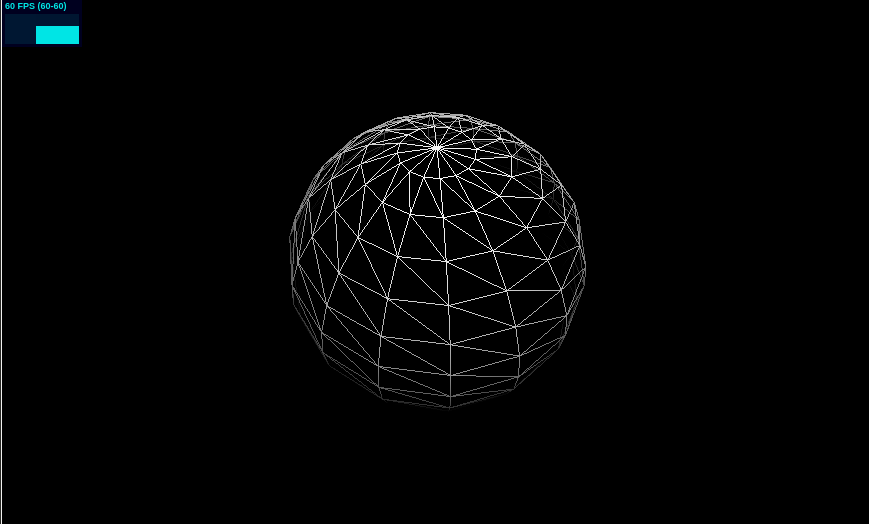
\includegraphics[width=1\linewidth]{images/sphere.png}

Para a renderização 3D, a biblioteca THREE.JS será utilizada.


\subsubsection{THREE.JS}

THREE.JS é uma biblioteca de JavaScript para a criação e execução de gráficos 3D em navegadores, de maneira leve e otimizada. Ele permite ao browser renderizar gráficos sem a necessidade de plugins, e utilizar a GPU \footnote{GPU (\emph{Graphics Processing Unit}) é um microprocessador especializado em processar gráficos. Sua estrutura de processamento paralelo os tornam mais capazes neste tipo de trabalho que CPUs normais. Uma GPU normalmente é utilizada em placas de vídeo.} do usuário para os cálculos de física e processamento de imagens. Essas funcionalidades são herdadas de WebGL, uma outra API de computação gráfica em JavaScript para browsers.

Sua interface é simples de se usar, ela lida internamente com os detalhes técnicos de implementação de baixo nível, deixando o desenvolvimento menos carregado, uma vez que processamento gráfico é uma área complexa da computação.

THREE.JS é completa o bastante para a criação de cenários 3D completos, com objetos, luzes e texturas. Por utilizar a GPU para o processamento, a performance não é comprometida por suas funcionalidades.

Abaixo está uma lista de funcionalidades que possui. Por possuir muitos termos inglês sem tradução em português, a lista de forma literal da sua página\footnote{https://en.wikipedia.org/wiki/Three.js} na Wikipédia:

\begin{itemize}

  \item \textbf{Effects}: Anaglyph, cross-eyed and parallax barrier.

  \item \textbf{Scenes}: add and remove objects at run-time; fog

  \item \textbf{Cameras}: perspective and orthographic; controllers: trackball, FPS, path and more

  \item \textbf{Animation}: armatures, forward kinematics, inverse kinematics, morph and keyframe

  \item \textbf{Lights}: ambient, direction, point and spot lights; shadows: cast and receive

  \item \textbf{Materials}: Lambert, Phong, smooth shading, textures and more

  \item \textbf{Shaders}: access to full OpenGL Shading Language (GLSL) capabilities: lens flare, depth pass and extensive post-processing library

  \item \textbf{Objects}: meshes, particles, sprites, lines, ribbons, bones and more - all with Level of detail

  \item \textbf{Geometry}: plane, cube, sphere, torus, 3D text and more; modifiers: lathe, extrude and tube

  \item \textbf{Data} loaders: binary, image, JSON and scene

  \item \textbf{Utilities}: full set of time and 3D math functions including frustum, matrix, quaternion, UVs and more

  \item \textbf{Export} and import: utilities to create Three.js-compatible JSON files from within: Blender, openCTM, FBX, Max, and OBJ

  \item \textbf{Support}: API documentation is under construction, public forum and wiki in full operation

  \item \textbf{Examples}: Over 150 files of coding examples plus fonts, models, textures, sounds and other support files

  \item \textbf{Debugging}: Stats.js, WebGL Inspector, Three.js Inspector
\end{itemize}


\newpage
\subsection{Servidor}

O servidor precisa ser projetado para escutar eventos do aplicativo, e responder ou encaminhar os dados recebidos. Ele será implementado com JavaScript, com o auxilio de Node.js e ExpressJS.

\subsubsection{Node.js e ExpressJS para criar um servidor}

Node.js é uma plataforma para desenvolvimento de aplicações \emph{server-side} (executadas no servidor) baseadas em rede utilizando JavaScript e o V8 JavaScript Engine \footnote{É o interpretador de JavaScript \emph{open source} implementado pelo Google em C++ e utilizado pelo Chrome.}. Com Node.js é possível criar aplicações Web utilizando apenas código em JavaScript.

Ao se levar em conta o modo em que o código em JavaScript pode ser estruturado e as demandas de aplicações Web, Node.js abre uma gama de novas possibilidades para desenvolvimento Web.

Express é um \emph{framework} mínimo e flexível para Node.js que oferece um conjunto robusto de funcionalidades. Sua API é simples, mas oferece ferramentas essenciais para o desenvolvimento de para páginas e aplicações Web e Mobile, e programas de \emph{backend}. Ela lida com detalhes de baixo nível como protocolos e processos. Além da sua funcionalidade básica, existem módulos disponíveis para adicionar novas, que são diretamente aplicados ao Express.


\newpage
\subsection{Exemplos de aplicações do modelo}

\begin{itemize}
    \item Com a base proposta pelo Projeto, a aplicação natural a ser desenvolvida seria um jogo virual. Para seu funcionamento, o smartphone serviria como o controle, e a execução do jogo seria na webpage.

    \begin{itemize}
        \item Uma ideia simples de jogo é utilizar o acelerômetro para calcular a inclinação do dispositivo e simular essa inclinação em um labirinto na webpage, guiar uma bola através dele com ajuda da gravidade.

        \item Outro exemplo mais tradicional é simular o layout de um controle na tela do dispositivo, quatro botões em cruz para setas e mais alguns para ações, e executar um jogo de plataforma na webpage.
    \end{itemize}

    \item É possível criar um aplicativo para supermercados. O consumidor usaria a câmera para consultar valores de produtos, recebendo-os do servidor do mercado. A webpage poderia ser apresentada no caixa, para que ele pudesse se atender sozinho, sem ajuda de funcionários.

    \begin{itemize}
        \item A webpage poderia ser utilizada também pela gerência, para ter um controle de quais produtos são mais requisitados ou quais possuem índices altos de desistência.
    \end{itemize}

    \item O smartphone pode ser utilizado para medir luz e ruído sonoro em um ambiente, e enviar esses valores para o servidor. A webpage pode exibir gráficos e estatísticas sobre essas leituras.

    \item A webpage pode exibir imagens, músicas, filmes ou vídeos. O smartphone serviria como um controle de multimídia, permitindo contolar volume, equalização de músicas, avançar ou voltar faixas ou filmes, pausar, entre outros. Além de ser um controle, o dispositivo também poderia exibir informações de contexto sobre a mídia exibida; caso seja um filme, mostra a sinopse, informações técnicas e atores.

    \item O modelo pode implementar um software para catalogar objetos. O smartphone pode tirar fotos e as enviar ao servidor, adicionar valores como nome, valor e tamanho. O servidor receberia essas tuplas e as inseriria em um bando de dados.

\end{itemize}








\newpage
\section{Implementação do caso de uso}

Nessa seção, é apresentada a implementação do caso de uso descrito para o Projeto, com o código exibido e explicado.

Em resumo, o caso de uso descreve o seguinte comportamento:

\begin{itemize}
    \item A webpage exibe uma esfera, em um ambiente em três dimensões. O servidor pode enviar valores à essa página, que irão rotacionar a esfera em seus eixos X, Y, Z. Esses valores também vão alterar a cor dessa esfera, de acordo com alguns cálculos.

    \item O servidor recebe dados do aplicativo e os envia para a webpage. Ele também envia feedbacks de volta ao aplicativo.

    \item O aplicativo controla o que acontece na webpage. Ele pode enviar eventos pontuais ou pode gerar um fluxo contínuo de valores do acelerômetro ao servidor.
\end{itemize}


\newpage
\subsection{Aplicativo}

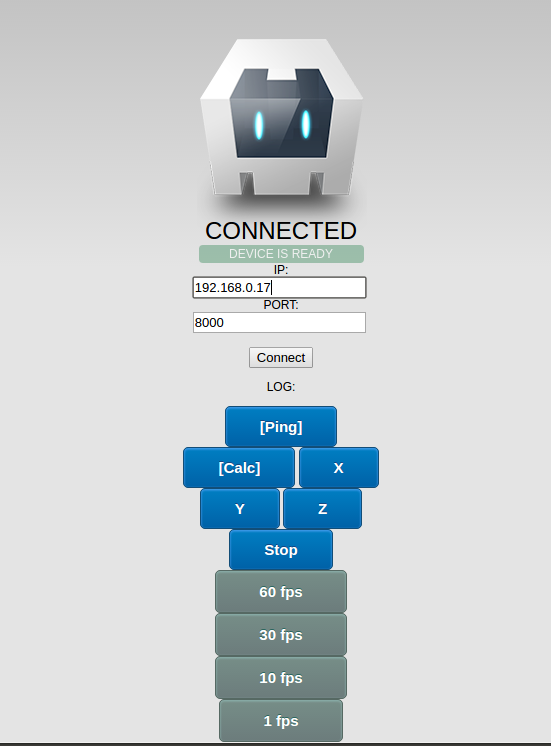
\includegraphics[width=1\linewidth]{images/Cordova.png}
\newpage


As interações da interface são:

\begin{itemize}
\item Um formulário para fazer a conexão com o servidor, dados IP e porta. Há um feedback visual que indica se ela foi bem sucedida.

\begin{itemize}
\item Uma vez conectado, o botão serve para fechar a conexão.
\end{itemize}

\item Um campo “Log" que exibe o resultado de algumas interações do usuário, ou mensagens enviadas do servidor.

\item Um conjunto de botões que emitem ações pontuais ao servidor, como calcular o \emph{Ping} \footnote{Tempo necessário para uma mensagem ser enviada ao servidor e voltar dele.} ou enviar um conjunto de dados.

\item Um outro conjunto de botões que ligam ou desligam um fluxo contínuo de mensagens. Essas mensagens emitidas contêm os dados do acelerômetro do dispositivo.

\begin{itemize}
\item Ao serem pressionados, esses botões iniciam o fluxo de mensagens. Se pressionados novamente, o fluxo é interrompido.
\end{itemize}

\end{itemize}

Essas funcionalidades implementadas já cobrem muitas interações desejadas no desenvolvimento de qualquer tipo de aplicativo.


\subsubsection{Código da Interface}
A parte visual do aplicativo está no arquivo index.html:


\begin{lstlisting}[language=HTML5]

<!DOCTYPE html>
<html>
    <head>
        <!-- <meta http-equiv="Content-Security-Policy" content="default-src 'self' data: gap: https://ssl.gstatic.com 'unsafe-eval'; style-src 'self' 'unsafe-inline'; media-src *;script-src 'self' http://cdn.socket.io/socket.io-1.0.3.js 'unsafe-inline' 'unsafe-eval'; connect-src localhost:*; "> -->

        <meta name="format-detection" content="telephone=no">
        <meta name="msapplication-tap-highlight" content="no">
        <meta name="viewport" content="user-scalable=no, initial-scale=1, maximum-scale=1, minimum-scale=1, width=device-width">
        <link rel="stylesheet" type="text/css" href="css/index.css">
        <link rel="shortcut icon" href="">
        <title>TCC</title>
    </head>
    <body>
        <div class="app">

            <h1 id="status">Disconnected</h1>
            <div id="deviceready" class="blink">
                <p class="event listening">Loading Device</p>
                <p class="event received">Device is Ready</p>
            </div>

            <form id="connect">
              IP:<br>
              <input type="text" name="ip" value="192.168.0.17">
              <br>
              Port:<br>
              <input type="text" name="port" value="8000">
              <br><br>
              <input id="connect" type="submit" value="Connect">
            </form>

            <p id="log">log:</p>

            <button class="btn" onclick="sendPing()">[Ping]</button>
            <button class="btn" onclick="localCalculation()">[Calc]</button>
            <button class="btn" onclick="addSpeed(speedX)">X</button>
            <button class="btn" onclick="addSpeed(speedY)">Y</button>
            <button class="btn" onclick="addSpeed(speedZ)">Z</button>
            <button class="btn" onclick="resetSpeed()">Stop</button>

            <button class="btn2" onclick="toggleAccelerometer(60)">60 fps</button>
            <button class="btn2" onclick="toggleAccelerometer(30)">30 fps</button>
            <button class="btn2" onclick="toggleAccelerometer(10)">10 fps</button>
            <button class="btn2" onclick="toggleAccelerometer(1)">1 fps</button>

        </div>
        <script type="text/javascript" src="cordova.js"></script>
        <script type="text/javascript" src="http://code.jquery.com/jquery-1.11.1.js"></script>
        <script type="text/javascript" src="http://cdn.socket.io/socket.io-1.0.3.js"></script>
        <script type="text/javascript" src="js/index.js"></script>
    </body>
</html>
\end{lstlisting}

\begin{itemize}
\item A divisão “deviceready" (linha 18) exibe o estado da conexão.

\begin{itemize}
\item Caso o dispositivo não tenha se conectado ainda, ele exibe “Connect Device".

\item Ao obter uma conexão bem sucessida com o servidor, ele muda para “Device is Connected".
\end{itemize}

\item O formulário “connect" (linha 23) faz a conexão do dispositivo com o servidor.

\begin{itemize}
\item Ele possui um campo para o IP e um para a Porta do servidor.

\item Ao apertar o botão “Connect", ele tenta fazer a conexão.
\end{itemize}

\item O parágrafo “log" (linha 33) exibe dados vindos do servidor.

\item Os botões (linha 35 a 45) executam diversas funções do código de enviar através de eventos para o servidor.

\item Os scripts (linha 48 a 51) importam as bibliotecas cordova, jquery e socket.io, e a parte lógica do aplicativo, encontrado em “js/index.js".
\end{itemize}


\subsubsection{Código da parte lógica}

A parte lógica do aplicativo está no arquivo index.js:


\begin{lstlisting}[language=JavaScript]
var app = {
    initialize: function() {
        this.bindEvents();
    },
    bindEvents: function() {
        document.addEventListener('deviceready', this.onDeviceReady, false);
    },
    onDeviceReady: function() {
        app.receivedEvent('deviceready');
    },
    receivedEvent: function(id) {
        var parentElement = document.getElementById(id);
        var listeningElement = parentElement.querySelector('.listening');
        var receivedElement = parentElement.querySelector('.received');

        listeningElement.setAttribute('style', 'display:none;');
        receivedElement.setAttribute('style', 'display:block;');

        console.log('Received Event: ' + id);
    }
};

app.initialize();


/*Variables */
var socket;
var watchID = null;

var speedX = {'x':1,'y':0,'z':0};
var speedY = {'x':0,'y':1,'z':0};
var speedZ = {'x':0,'y':0,'z':1};


/* Auxiliar functions */
function log(message) {
    socket.emit('device_print', message);
    var msg = 'Log: ' + message;
    $('#log').text(msg);
}

function validateIPaddress(ipaddress) {
    if (/^(25[0-5]|2[0-4][0-9]|[01]?[0-9][0-9]?)\.(25[0-5]|2[0-4][0-9]|[01]?[0-9][0-9]?)\.(25[0-5]|2[0-4][0-9]|[01]?[0-9][0-9]?)\.(25[0-5]|2[0-4][0-9]|[01]?[0-9][0-9]?)$/.test(ipaddress)) {
    // if (/^192\.168?\.(25[0-5]|2[0-4][0-9]|[01]?[0-9][0-9]?)\.(25[0-5]|2[0-4][0-9]|[01]?[0-9][0-9]?)$/.test(ipaddress)) {
        return (true)
    }
    log("You have entered an invalid IP address!")
    return (false)
}

function toggleAccelerometer(period) {
    var freq = ~~(1000 / period);
    if (watchID == null) {
        watchID = navigator.accelerometer.watchAcceleration(
            sendAcceleration,
            sendAccError,
            { frequency: freq }
        );
        navigator.accelerometer.getCurrentAcceleration(sendAcceleration, sendAccError);
    }
    else {
        navigator.accelerometer.clearWatch(watchID);
        watchID = null;
    }
}


/* Socket emit functions */
function addSpeed(speed_vector) {
    socket.emit('device_add_speed', speed_vector);
}

function resetSpeed() {
    socket.emit('device_reset_speed');
}

function sendAcceleration(acceleration) {
    socket.emit('device_acceleration', acceleration)
}

function sendAccError() {
    log('Accelerometer error.');
}

function sendPing() {
    var timestamp = Date.now();
    socket.emit('device_ping', timestamp);
}

function localCalculation() {
    var t0 = Date.now();
    var r = 0;
    var i, j, k;
    for(i = 0; i < 1000000; i++) {
        for(i = 0; i < 10000000; i++) {
            for(i = 0; i < 10000000; i++) {
                r += (3 * i + (j + k / 2))% 103;
            }
        }
    }

    var t1 = Date.now();
    socket.emit('request_calculation');
    log('Finished device calculation in ' + (t1 - t0));
}


/*Socket events */
function onServerConnect() {
    $('#status').text("Connected");
    app.receivedEvent('deviceready');
    socket.emit('ready', 'device');
}

function onServerPing(data) {
    var dt = Date.now() - data.t0;
    log('Ping: ' + dt);
}

function onServerLog(msg) {
    $('#log').text(msg);
}

function connectSocket(ipaddress, port) {
    if(validateIPaddress(ipaddress)) {
        if(socket !== null && socket !== undefined) {
            socket.emit('device_disconnected');
            socket.disconnect();
            $('#status').text("Disconnected");
        }
        else{
            socket = io('http://' + ipaddress + ':' + port);

            socket.on('connect', onServerConnect);
            socket.on('server_ping', onServerPing);
            socket.on('device_log', onServerLog);
        }
    }
}


/*Device Ready Event */
document.addEventListener('deviceready', function() {

    $('#connect').submit(function (event) {
        var ip   = this.ip.value;
        var port = this.port.value;

        connectSocket(ip, port);

        return false;
    });
});

\end{lstlisting}

\textbf{Para inicializar o aplicativo:}

\begin{itemize}
  \item A variável \code{app} é uma classe padrão do Cordova com funções para inicializar o aplicativo. Ele é inicializado na linha 23.
\end{itemize}


\textbf{Para fazer a conexão com o servidor:}

\begin{itemize}
  \item Na linha 143, uma função é adicionada ao evento \emph{“deviceready"} que o Cordova emite quando toda a inicialização é finalizada. Na ocorrência desse evento, a ação do botão “Connect" é alterada para tentar conectar-se ao servidor, através da função \code{connectSocket}.

Essa função \code{connectSocket} recebe o IP e Porta vindos do formulário do botão. Se o IP for válido (a função \code{validateIPaddress} faz essa verificação com expressões regulares), ela fazer uma conexão entre o dispositivo e o servidor definido por esses IP e Porta. Se a conexão já está feita, ele a disconecta.
\end{itemize}

\textbf{Eventos que o servidor ativa:}
\begin{itemize}
  \item Na inicialização do Socket, três eventos são definidos: \emph{“connect"} chama a função \code{onServerConnect}; \emph{“server\_ping"} chama \code{onServerPing} e  \emph{“device\_log"} chama \code{onServerLog}.

  \item \code{onServerConnect} : Emite ao socket um evento \emph{“ready"} para o servidor para informar o seu tipo e atualiza informações exibidas.

  \item \code{onServerPing}: Calcula o \emph{ping} que foi enviado.

  \item \code{onServerLog}: Exibe na tela a mensagem recebida, no campo \emph{LOG}.
\end{itemize}


\textbf{Eventos enviados ao servidor:}
\begin{itemize}
  \item As funções \code{addSpeed}, \code{resetSpeed}, \code{sendAcceleration}, \code{sendPing} e \code{localCalculation} enviam mensagens ao servidor com dados obtidos do input do usuário ou leitura do smartphone.

  \item A função \code{toggleAccelerometer} ativa um loop que manda leituras do acelerômetro em intervalos regulares.
\end{itemize}



\newpage
\subsection{Webpage}

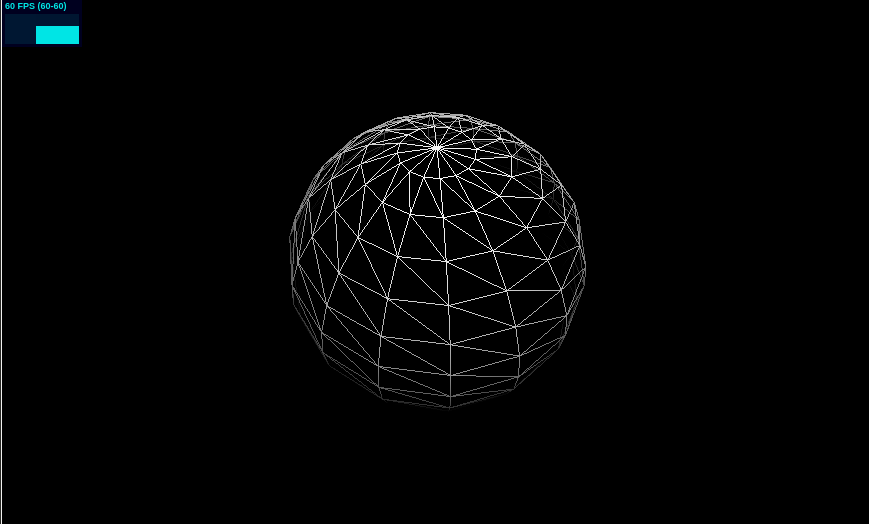
\includegraphics[width=1\linewidth]{images/sphere.png}

Essa página explora somente o básico de THREE.js para a criação de um ambiente 3D.

Este código é mais extenso, então somente as partes principais são exibidas.

O primeiro arquivo, \code{global.js}, declara variáveis globais, usadas em mais de um módulo:


\begin{lstlisting}[language=JavaScript]
var socket;

var xRot, yRot, zRot;
var r, g, b;
var hasNewColors;
\end{lstlisting}

As variáveis declaradas definem o seguinte:

\begin{itemize}
  \item O socket da conexão;

  \item As velocidades de rotação \code{xRot}, \code{yRot} e \code{zRot};

  \item A cor RGB da esfera;

  \item Uma \emph{flag} que aponta se a cor precisa ser atualizada.
\end{itemize}


O arquivo \code{socket\_events.js}, define os eventos escutados e seus \emph{callbacks}:


\begin{lstlisting}[language=JavaScript]
socket = io();

function rotate (data) {
    xRot += data.x;
    yRot += data.y;
    zRot += data.z;
}

function reset_rotation () {
    xRot = 0;
    yRot = 0;
    zRot = 0;
}

function update_rotation_and_colors (data) {
    var cap = 9;
    var x = Math.min(data.x, cap);
    var y = Math.min(data.y, cap);
    var z = Math.max(2, Math.min(data.z, cap));

    var weight = 5;

    xRot = y / 50;
    yRot = x / 50;

    r = (weight * r + (z / cap)) / (weight + 1);
    g = (weight * g + (z / cap)) / (weight + 1);
    b = (weight * b + (z / cap)) / (weight + 1);

    hasNewColors = true;
}

// Socket Events

socket.on('connect', function() {
    socket.emit('ready', 'browser');
});

socket.on('move', function (data) {
    rotate(data);
});

socket.on('reset', function () {
    reset_rotation();
});

socket.on('update_acceleration', function (data) {
    update_rotation_and_colors(data);
})
\end{lstlisting}

Há 4 eventos de Sockets:

\begin{itemize}

  \item \emph{“connect"}: Ao se conectar, emite um evento \emph{“ready"} com seu tipo.

  \item \emph{“move"}: Recebe valores X, Y e Z, e os associa à velocidade de rotação da esfera em cada um desses eixos. Essa associação é incremental, a velocidade aumenta a cada evento.

  \item \emph{“reset"}: Zera as velocidades de rotação da esfera.

  \item \emph{“update\_acceleration"}: Recebe valores X, Y, Z que definem a velocidade de rotação total da esfera (não incremental). Também altera sua cor incrementalmente, de acordo com alguns cálculos com as variáveis.

\end{itemize}

Por fim, o arquivo \code{three\_sphere.js} cria cria todos os elementos gráficos e os renderiza.

\begin{lstlisting}[language=JavaScript]
var scene, camera, renderer;
var sphere, sphere;

hasNewColors = false;

function updateSphereRotation(xRot, yRot, zRot) {
    sphere.rotation.x += xRot;
    sphere.rotation.y += yRot;
    sphere.rotation.z += zRot;
}

function updateSphereColor(r, g, b) {
    sphere.material.color.r = r;
    sphere.material.color.g = g;
    sphere.material.color.b = b;
}


function init() {

    scene = new THREE.Scene();

    var view_angle = window.innerWidth/window.innerHeight
    camera = new THREE.PerspectiveCamera( 75, view_angle, 0.1, 1000 );
    camera.position.z = 5;
    scene.add(camera);

    renderer = new THREE.WebGLRenderer();
    renderer.setSize( window.innerWidth, window.innerHeight );
    document.body.appendChild( renderer.domElement );

    //-------------------------------------------

    // create a point light
    var pointLight = new THREE.PointLight(0xFFFFFF);

    // set its position
    pointLight.position.x = 10;
    pointLight.position.y = 50;
    pointLight.position.z = 130;

    // add to the scene
    scene.add(pointLight);

    //-------------------------------------------

    // New Sphere
    var radius = 2;
    var segments = 16;
    var rings = 16;

    var sphereGeo = new THREE.SphereGeometry(radius, segments, rings);
    var sphereMaterial = new THREE.MeshLambertMaterial( {
        color: 0xCC0000,
        wireframe : true
    } );
    sphere = new THREE.Mesh( sphereGeo, sphereMaterial );
    scene.add( sphere );

    //-------------------------------------------

    xRot = 0;
    yRot = 0;
    zRot = 0;

    r = 1;
    g = 1;
    b = 0;
}

function render() {
    requestAnimationFrame( render );

    updateSphereRotation(xRot, yRot, zRot);
    if (hasNewColors) {
        updateSphereColor(r, g, b);
        hasNewColors = false;
    };

    renderer.render(scene, camera);
};

init();
render();
\end{lstlisting}

\begin{itemize}
  \item \code{init()} cria os elementos do cenário: a cena, a camera, o renderizador, a iluminação e a esfera, além de inicializar as variáveis.

  \item \code{render()} atualiza a posição da esfera de acordo com sua velocidade (com \code{updateSphereRotation()}), sua cor (com \code{updateSphereColor()}), caso haja mudanças, e renderiza a cena. Essa função é chamada a cada \emph{frame}, o que garante que a esfera seja animada.
\end{itemize}



\newpage
\subsection{Servidor}

O servidor criado tem suas configurações definidas no arquivo \code{package.json}. Esse arquivo permite a restauração e reprodução do servidor em outros locais.


\begin{lstlisting}[language=JavaScript]
{
  "name": "socket.io-server_aplication",
  "version": "0.9.0",
  "description": "A client manager using socket.io",
  "main": "index.js",
  "author": "Guilherme Freire Silva",
  "private": true,
  "license": "BSD",
  "dependencies": {
    "express": "4.13.4",
    "socket.io": "^1.4.8"
  }
}

\end{lstlisting}

\begin{itemize}
  \item A configuração mais importante para a reprodução é a de dependencias, na qual estão definidas \code{express} e \code{socket.io}.
\end{itemize}

Para a leitura do código, é importante ter em mente que o servidor faz uma distinção entre sockets de \emph{browser}, que executam a aplicação Web, e sockets de \emph{device}, que executam o aplicativo do Cordova.

O código que cria o servidor está em \code{index.js}:

\begin{lstlisting}[language=JavaScript]
// Setup basic express server
var express = require('express');
var app     = express();
var server  = require('http').createServer(app);
var io      = require('socket.io')(server);
var port    = 8000;

server.listen(port, function () {
    console.log('Server listening at port %d', port);
});

// Routing
app.use(express.static(__dirname + '/public'));



// -------------------------------------

var device_dict  = {};
var browser_dict = {};

// Function to send (event, data) only to browser sockets
function emit_to_browser_socket(event, data) {
    for (var key in browser_dict) {
        if (browser_dict[key].connected) {
            browser_dict[key].emit(event, data);
        }
        else {
            console.log("  > Disconnected socket!")
            delete browser_dict[key];
        }
    }
}

io.on('connection', function (socket) {

    socket.on('ready', function (data) {
        if (data == 'device') {
            console.log('device  connected:', socket.id);
            device_dict[socket.id] = socket;
        }
        else if (data == 'browser'){
            console.log('browser connected:', socket.id);
            browser_dict[socket.id] = socket;
        }
    })

    // -------------------------------------
    // Device events

    socket.on('device_ping', function (sent) {
        var received_in_server = Date.now();
        socket.emit('server_ping', {
            t0 : sent,
            t1 : received_in_server
        });
    });

    socket.on('device_add_speed', function (data) {
        console.log('device_add_speed', data);
        emit_to_browser_socket('move', data)
    });

    socket.on('device_reset_speed', function () {
        console.log('device_reset_speed');
        socket.emit('device_log', 'server: reset speed');
        emit_to_browser_socket('reset', {})
    });

    socket.on('device_print', function (data) {
        console.log(data);
    })

    // Expected Structure: { x: -0.39, y: 0.06, z: 0.2, timestamp: 1476064230489 }
    socket.on('device_acceleration', function (data) {
        emit_to_browser_socket('update_acceleration', data)
    })


    // -------------------------------------
    // Client events

    // Echo browser > server > browser
    socket.on('echo_move', function (data) {
        socket.emit('move', data);
    });
});
\end{lstlisting}


O servidor é criado utiliznado o ExpressJS, ouvindo na porta definida e utilizando recursos encontrados na pasta \code{/public}.

Quando uma conexão é iniciada, o socket criado é atribuído de eventos e seus respectivos \emph{callbacks}. Os eventos são:

\begin{itemize}

    \item \emph{'ready'}: Ocorre logo após a conexão ser iniciada. O cliente envia qual o seu tipo, e o servidor o insere em um dicionário de \emph{devices} ou de \emph{browsers}, indexado pelo \emph{id} desse socket.

    \item \emph{'device\_ping'}: É a metade do caminho do \emph{Ping} lançado pelo \emph{device}. Essa função emite um evento \emph{'server\_ping'} de volta ao \emph{device}, com o \code{timestamp} recebido e o atual.

    \item \emph{'device\_add\_speed'}: Recebe um conjunto de valores X, Y e Z, e os emite para todos os \emph{browsers}, com o evento \emph{'move'}.

    \item \emph{'device\_reset\_speed'}: Emite um evento \emph{'device\_log'} para o \emph{device} logar na sua tela, e emite um evento \emph{'reset'} aos \emph{browsers} sem dados. Esse evento é usado para parar a rotação da esfera.

    \item \emph{'device\_print'}: É uma função de \emph{debug}. Somente imprime no console os dados recebidos.

    \item \emph{'device\_acceleration'}: Recebe os dados do acelerômetro do \emph{device} e os emite aos \emph{browsers} com um evento \emph{'update\_acceleration'}.

    \item \emph{'echo\_move'}: Recebe do \emph{browser} um valor de aceleração X, Y e Z, e emite de volta pelo evento \emph{'move'}.

    \item Há uma função auxiliar \code{emit\_to\_browser\_socket(event, data)} que emite o evento \emph{'event'} com a mensagem \emph{'data'} para todos os sockets de \emph{'browsers'}.

\end{itemize}


\newpage
\section{Teste e avaliação}

Esse capítulo descreve os resultados da implementação do caso de uso acima.


\subsection{Comunicação via Socket.io}

A conexão foi testada durante todos os momentos do desenvolvimento, desde o momento da sua implementação. O teste foi feito somente em redes locais, pois implementar segurança para conexão em qualquer endereço estava fora do escopo.

Na maior parte dos testes, a rede WiFi local não era dividida por vários dispositivos, na prática era exclusiva do servidor e do smartphone.

Foram utilizados dois smartphones para os testes:
\begin{itemize}
    \item Dispositivo A : LG G2
    \item Dispositivo B : Moto Z
\end{itemize}

Aqui estão lembretes de funcionalidades implementadas:

\begin{itemize}

    \item \textbf{Ping}: Essa função envia um evento ao servidor e espera um evento de resposta, para calcula o tempo entre o envio e a chegada.

    \item \textbf{Fluxo de Eventos}: Foram implementados botões para ligar ou desligar um fluxo constante de eventos ao servidor, a intervalos regulares. Os intervalos são:
    \begin{itemize}
        \item 60 vezes por segundo.
        \item 30 vezes por segundo.
        \item 10 vezes por segundo.
        \item 1 veze por segundo.
    \end{itemize}

    \item \textbf{Cálculo Local}: Há uma função de cálculo, presente tanto no aplicativo como no servidor. É calculado o tempo que cada dispositivo leva para fazê-lo, para comparar a eficiência entre eles.

    A função é a seguinte:
    \begin{lstlisting}[language=JavaScript]
    var r = 0;
    var i, j, k;
    for(i = 0; i < 1000000; i++) {
        for(i = 0; i < 10000000; i++) {
            for(i = 0; i < 10000000; i++) {
                r += (3 * i + (j + k / 2))% 103;
            }
        }
    }
    \end{lstlisting}

\end{itemize}

De volta aos testes, os pontos que merecem ser citados:

\begin{itemize}

    \item Uma conexão é feita entre o smartphone e o servidor. Nesse momento, enquanto os dois processos estão em repouso, foram executadas chamadas à função de Ping.

    \begin{itemize}
        \item \textbf{Resultado A}: valores variavam bastante entre \textbf{15 milissegundos} e \textbf{120 milissegundos}. Poucos valores saíam desse intervalo, a média era de \textbf{65 milissegundos}, aproximadamente.
        \item \textbf{Resultado B}: valores variavam bastante entre \textbf{15 milissegundos} e \textbf{120 milissegundos}. Poucos valores saíam desse intervalo, a média era de \textbf{65 milissegundos}, aproximadamente.
    \end{itemize}

    \item O teste acima foi refeito, com o Fluxo de Eventos ligado a 60 e 30 vezes por segundo.

    \begin{itemize}
        \item \textbf{Resultado A}: Muito contra intuitivamente, o tempo de ping caiu para para um intervalo de \textbf{1 a 5 milissegundos}.
        \item \textbf{Resultado B}: Muito contra intuitivamente, o tempo de ping caiu para para um intervalo de \textbf{1 a 5 milissegundos}.
    \end{itemize}


\end{itemize}









%%%%%%%%%%%%%%%%%%%%%%%%%%%%%%%%%%%%%%%%%%%%%%%%%%%%%%%%%%%%%%%%%%%
%%%%%%%%%%%%%%%%%%%%%%%%%%%%%%%%%%%%%%%%%%%%%%%%%%%%%%%%%%%%%%%%%%%
%%%%%%%%%%%%%%%%%%%%%%%%%%%%%%%%%%%%%%%%%%%%%%%%%%%%%%%%%%%%%%%%%%%
%
% FIM DA SESSÃO ~~~~~~~~~~~~~~~~~~~~~~~~~~~~~~~~~~~~~~~~~~~~~~~~~~%
%
%%%%%%%%%%%%%%%%%%%%%%%%%%%%%%%%%%%%%%%%%%%%%%%%%%%%%%%%%%%%%%%%%%%
%%%%%%%%%%%%%%%%%%%%%%%%%%%%%%%%%%%%%%%%%%%%%%%%%%%%%%%%%%%%%%%%%%%
%%%%%%%%%%%%%%%%%%%%%%%%%%%%%%%%%%%%%%%%%%%%%%%%%%%%%%%%%%%%%%%%%%%








\newpage

\section{Estudo Aprofundado da Tecnologia}

\subsection{Desenvolvendo Aplicativos com Apache Cordova}

O Apache Cordova é um \emph{framework} \emph{open-source} para a criação de aplicativos para \emph{mobile}. Seu desenvolvimento é dado com o uso de tecnologias Web, como HTML5, CSS3 e JavaScript.

Ele é multiplataforma, permite o desenvolvimento para sistemas como Android, iOS ou navegadores. Por tal motivo, oferece uma API de alto nível para acessar os módulos desejados, tais como de sensores, arquivos e rede. A interface para o uso dessas funcionalidades é abstrata, de forma que código desenvolvido é executável em todas as plataformas oferecidas e o desenvolvedor não precisa se preocupar com os detalhes de cada uma na hora da implementação.

O aplicativo implementado é uma exatamente página Web, a estrutura é a mesma. Há um arquivo principal “index.html" que referencia os recursos necessários, como CSS, JavaScript, imagens e arquivos de mídia. A parte lógica é feita em JavaScript, e a renderização em HTML5 e CSS3. Para ser portado para uma plataforma específica, o HTML é enviado para a classe \emph{“Wrapper”} dessa plataforma, onde estão definidos os detalhes de implementação. Essa classe também tem incorporada um browser nativo, o \emph{WebView}, que executará o programa Web dentro do dispositivo.

A comunicação entre o aplicativo e os componentes nativos de cada plataforma é dada a partir de Plugins instalados. Cada Plugin é uma biblioteca adicional que permite ao \emph{WebView} interagir com funcionalidades da plataforma nativa na qual está rodando. Eles provêm acesso a essas funcionalidades normalmente não disponíveis em aplicativos Web. Essas ferramentas são disponibilizadas para o desenvolvedor através de uma expansão da API inicial, que toma para si os detalhes da implementação em cada plataforma, simplificando o desenvolvimento.

Há um conjunto principal de Plugins, chamado de \emph{Core}, que é mantido pelo próprio Cordova. Nele estão contidos os que acessam as principais funcionalidades de um dispositivo mobile, como acesso ao acelerômetro, câmera, bateria e geolocalização.

Há também Plugins desenvolvidos por terceiros (em geral pela própria comunidade) que trazem relações com outras funcionalidades, talvez exclusivas de uma plataforma. Enquanto no \emph{Core} há apenas umas poucas dezenas, a lista de Plugins criada pela comunidade oferece centenas com as mais diversas funcionalidades, como um para compras dentro do App e um para enviar notificações para dispositivos vestíveis (Smartwatches, por exemplo). A criação de um Plugin é simples e incentivada, no site do Cordova há um tutorial.

O método de desenvolvimento descrito até agora, focado em várias plataformas, é um dentre dois possíveis \emph{Workflows} disponíveis no Cordova e seu nome é \emph{“Cross-platform”} (CLI). Ele deve ser usado se o aplicativo desenvolvido pretende alcançar a maior variedade de Sistemas Operacionais \emph{mobile}, com pouca ou nenhuma ênfase no desenvolvimento em uma plataforma específica.

O segundo \emph{Workflow} é chamado \emph{“Platform-centered”}, e deve ser usado se o projeto é focado para uma única plataforma e se pretende modificá-la em baixo nível.

A arquitetura interna está descrita no diagrama:

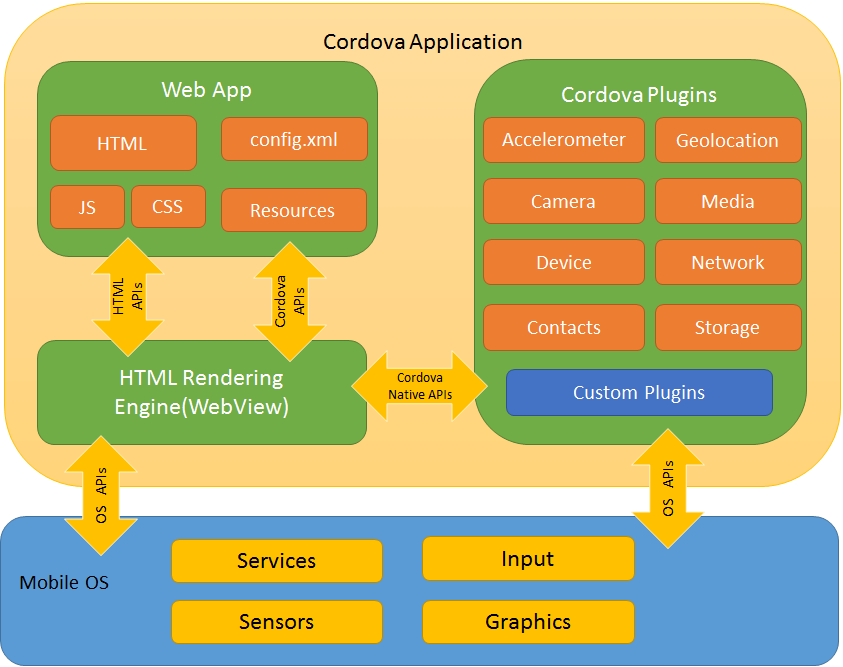
\includegraphics[width=1\linewidth]{images/cordovaapparchitecture.png}



% \newpage
% \subsection{Utilizando Node.js e ExpressJS}

% *Something Something*

% % https://www.tutorialspoint.com//nodejs/nodejs_introduction.htm
% Alguns atributos chave de Node.js são:

% % Asynchronous and Event Driven − All APIs of Node.js library are asynchronous, that is, non-blocking. It essentially means a Node.js based server never waits for an API to return data. The server moves to the next API after calling it and a notification mechanism of Events of Node.js helps the server to get a response from the previous API call.
% - Assíncrono e Orientado a Eventos - Todas as APIs da biblioteca de Node.js são assíncronas, o que garante que são não bloqueantes. Isso essencialmente significa que um servidor baseado em Node.js não espera por dados de retorno da chamada da API, ele somente continua com sua execução para a próxima chamada de API. Os dados de retorno chegam ao servidor atráves de um mecanismo de notificações, os Eventos de Node.js. % Cada evento ativa um callback para os dados serem tratados.


% % Very Fast − Being built on Google Chrome's V8 JavaScript Engine, Node.js library is very fast in code execution.
% - Muito rápido - Por ser construído com base no V8 JavaScript Engine do Google Chrome, a biblioteca de Node.js é muito veloz em execução de código.

% % Single Threaded but Highly Scalable − Node.js uses a single threaded model with event looping. Event mechanism helps the server to respond in a non-blocking way and makes the server highly scalable as opposed to traditional servers which create limited threads to handle requests. Node.js uses a single threaded program and the same program can provide service to a much larger number of requests than traditional servers like Apache HTTP Server.
% - Possui \emph{thread} única porém é muito escalável - Node.js possui um modelo de laço de Eventos com a utilização de uma única \emph{thread}. O mecanismo de Eventos ajuda o servidor enviar respostas de forma não bloqueante e faz o seridor altamente escalável em comparação ao modelo tradicional de servidores que criam um número limitado de \emph{threads} para lidar com requisições dos clientes. Node.js usa um programa de \emph{thread} única e esse mesmo programa pode providenciar serviço a um número muito maior de requisições do que um servidor tradicional, como o Apache HTTP.

% % No Buffering − Node.js applications never buffer any data. These applications simply output the data in chunks.
% - Sem \emph{Buffering} - Aplicações em Node.js nunca armazenam nenhum dado em \emph{buffers}. Essas apliações simplesmente enviam dados em blocos.

% % License − Node.js is released under the MIT license.
% - Licenciado - Node.js está sob uma licença MIT.



\newpage
\subsection{Comunicação Web e Aplicações Web}


O protocolo WebSocket foi utilizado para a comunicação deste Projeto, pois há vários fatores no protocolo HTTP e do modelo cliente-servidor convencional que se tornam empecilhos para as necessidades apresentadas.

Enquanto que, na prática, bastou escolher esse protocolo WebSocket, sua criação representa uma evolução no paradigma de desenvolvimento de páginas Web. A seguir é dado um panorama dos fatores que desencadearam sua criação e o que isso representa.


% cliente-servidor
\subsubsection{Modelo cliente-servidor}

A comunicação de dados entre computadores através da Internet é algo muito comum, e necessita de uma arquitetura de rede adequada para ocorrer.

A mais utilizada é o modelo cliente-servidor. Neste modelo, existem dois tipos de processos rodando, o Cliente e o Servidor. O Cliente é o processo que roda nos computadores locais e se conecta ao Servidor. A comunicação é dada quando o Cliente manda uma requisição ao Servidor (esta requisição pode ser por uma página web, um processamento de dados, entre outros). Por sua vez, o Servidor recebe esses dados e faz o processamento necessário para completar essa requisição, e em seguida envia uma resposta ao Cliente. A resposta pode pode ser o que foi requisitado ou outro tipo de mensagem, como de erro, caso ocorra uma falha no processamento ou negação de permissão. O Cliente então pode continuar com o seu próprio processo.


% HTTP
%\subsubsection{Protocolo HTTP}

O protocolo que acompanha esse modelo é principalmente HTTP (\emph{Hypertext Transfer Protocol}). Ele é usado para a transferência de Recursos entre processos. Recursos são arquivos HTML, imagens, resultados de buscas, entre outros.

Um Cliente HTTP, como um navegador, abre uma conexão e envia uma mensagem de requisição ao Servidor HTTP, que retorna uma mensagem de resposta, normalmente contendo o recurso pedido. Após entregar a resposta, o Servidor encerra a conexão.

Por encerrar a conexão, é dito que HTTP um protocolo sem estado, pois não mantém informações sobre a conexão entre transações. Ele também implica que cada mensagem HTTP precisa possuir um cabeçalho com informações sobre o contexto, uma vez que o Servidor não guarda nenhum dado.





% (TODO nota de rodapé)
% P2P
% A outra grande arquitetura muito utilizada também é a peer-to-peer (P2P). Nessa arquitetura, não há um computador central para funcionar como servidor, cada computador conectado (Peer) na rede realiza funções tanto de cliente como de servidor na aplicação que está sendo executada. Essa aplicação tem suas tarefas organizadas e divididas entre os Peers.
% Essa arquitetura é conhecida principalmente por ser usada para a transferência de arquivos grandes, como músicas e vídeos. Nessa transmissão, os Peers que tem o arquivo são conectados aos que não tem, e começam a transferência de pequenos pacotes de dados. Esses pacotes não precisam vir ordenados e o Peer receptor os armazena localmente. Uma vez que a transferência é completada, ele ordena os pacotes e monta o arquivo final. Uma vantagem dessa arquitetura é que a tranferência não é limitada pela capacidade de banda de Servidor, e Peers podem se conectar e desconectar sem que haja problemas para o receptor, o arquivo são será corrompido por eventuais problemas de conexão. Um ponto negativo é que, sem um Servidor, não há um controle de que tipos de arquivos estão sendo transferidos (o que abre uma porta para pirataria) e não é fácil interromper uma transferência, uma vez que ela pode ser composta de milhares de conexões. Outro ponto é que não é fácil de se conhecer a procedência dos dados recebidos, a segurança não pode ser garantida.

% Esta arquitetura não serve para as necessidades do projeto, a hipótese de uso foi descartada após o estudo de sua estrutura.



%Começo de problemas em usar somente cliente-servidor
O modelo cliente-servidor é suficiente para páginas Web, pois o Cliente pede páginas estáticas e o Servidor as fornece sempre que necessário. Mas essa arquitetura não permite um uso mais dinâmico dessas páginas Web, pois sua estrutura é muito burocrática.

Para fazer uma página mais responsiva, com \emph{feedbacks} a cada ação do usuário e dados novos, seria necessário que o Cliente fizesse uma requisição ao Servidor após cada ação executada (como preencher um formulário ou levar o cursor a algum ponto específico, por exemplo). Cada requisição HTTP dessas carregaria muitas informações em seu cabeçalho. Ao receber a página atualizada, o Cliente ainda precisaria recarregá-la para atualizar o que fosse necessário. Os dois problemas claros nessa estrutura são:

\begin{itemize}
    \item A necessidade de recarregar a página inteira, mesmo que somente uma pequena parcela dos dados tenha sido alterada. Esse comportamento foi criado em um momento no qual não se tinha a necessidade de alterar pequenas coisas na página, e que cada HTML vindo do Servidor seria uma página completamente nova. A impossibilidade de atualizar dados individualmente remove qualquer dinamicidade desejada.

    \item O \emph{overhead} gerado pelo cabeçalho das mensagens HTTP. Esse \emph{overhead} cria uma latência (tempo de resposta) alta e faz com que um envio contante de requisições ao Servidor exija muitos recursos.
\end{itemize}

Um exemplo de comportamento impossível com essas restrições é dar um \emph{feedback} instantâneo para o usuário na hora que ele está preenchendo um cadastro em algum site, como informar se o email inserido já foi usado ou se a senha possui os parâmetros mínimos necessários de segurança.

% Apresento Ajax
\subsubsection{AJAX}

Da discussão gerada a partir desses problemas surgiu o Ajax (\emph{Asynchronous JavaScript and XML}). Ajax é uma técnica de desenvolvimento Web criada para possibilitar a requisição por dados parciais ao Servidor e recebê-los de forma assíncrona no \emph{background}, sem precisar recarregar a página exibida. Com essa técnica passa a ser possível atualizar partes de uma página com base em eventos do usuário.

% Exemplo de Ajax
Para ilustrar esse funcionamento com um exemplo simples, basta usar a ferramenta de busca do Google\footnote{google.com}. O usuário começa a digitar uma busca e resultados já aparecem sem a necessidade de atualizar a página, mesmo antes da busca estar completa. O \emph{input} do usuário ativa requisições no \emph{background} para obter e atualizar os resultados exibidos, sem se preocupar se a busca será alterada no futuro. Assim, o usuário recebe um \emph{feedback} mais dinâmico e menos burocrático do que o convencional (digitar a busca completa e ir para uma página de resultados).

% Final de Ajax
Com o Ajax, nota-se uma mudança de paradigmas na Web. Onde antes só havia a noção de página Web, agora começa a se formar uma noção de Aplicação Web. Antes, a maior interatividade possível era algo como um fluxo de telas com dados dependentes da tela passada, mas agora ações de usuários passam a ter resultados instantâneos. Sites com um fluxo de dados muito grande e dinâmico passam a ser possíveis, como Facebook \footnote{facebook.com}, no qual é possível fazer comentários, interagir com usuários e visualizar tanto conteúdo quando desejado sem precisar atualizar a página.

% Começo da necessidade de comunicação bilateral
Essa mudança de paradigmas fez com que muitas Aplicações tipicamente executadas em \emph{Desktop} fossem desenvolvidas para Web, como clientes de email ou aplicações que exigissem um fluxo de dados muito grande entre o Cliente e o Servidor. Mas o que ficou claro com o tempo é que Ajax não bastava para muitas dessas Aplicações, em específico as que funcionavam em tempo real. Muitas vezes é o Servidor que precisa se comunicar ao Cliente sobre mudança nos dados. O modelo de funcionamento do Ajax não possui esse tipo de interface, então, para fazer aplicações assim funcionarem corretamente, é necessário muito esforço, lutar contra a linguagem.

% Exemplo da necessidade de comunicação bilateral
Um exemplo claro disso é uma aplicação de \emph{Chat}. Não é possível ter um padrão de quando o Servidor tem novas mensagens, então é necessário que o Cliente faça requisições a cada período de tempo. Se esse período for curto, o fluxo de dados intenso pode se tornar um problema. Se o período for longo, vai contra o princípio de ser uma comunicação em tempo real, mensagens vão demorar mais a serem entregues. Além disso, o modelo de comunicação do Ajax envia e recebe mensagens em paralelo, sem preservar sua ordem. Então, ao se fazer atualizações síncronas, é necessário ainda um tratamento de ordenação para exibir as mensagens novas.

% Conclusão Ajax e necessidade de CommBi
A necessidade de vários tratamentos para uma aplicação relativamente simples funcionar deixou claro que havia necessidade de mais ferramentas para o desenvolvimento de aplicações Web.


\subsubsection{Necessidade de Comunicação Bilateral}

% Maneiras de simular CommBi
Um dos fatores mais limitantes era que a comunicação cliente-servidor não é bilateral. Não é possível para o Servidor mandar dados espontaneamente, sem que o Cliente tenha feito uma requisição antes. Para contornar esse problema foram criadas técnicas para simular essa comunicação bilateral: \emph{Polling}, \emph{Long-Polling} e \emph{Streaming}.


\begin{itemize}

    \item \textbf{Polling}

    Essa técnica já foi descrita acima no exemplo do \emph{Chat}. Ela consiste em fazer o Cliente mandar requisições em intervalos regulares e receber a resposta logo em seguida. Ela foi a primeira tentativa de se contornar o problema, principalmente por ter a implementação mais simples e direta.

    Essa solução é boa quando se sabe o tempo de atualização de dados no Servidor, pois é possível sincronizar os tempos de requisição e atualização. Porém esse é somente um dos cenários possíveis. Dados em tempo real não costumam ser tão previsíveis, então é inevitável que uma parcela dessas requisições seja desnecessária e muitas conexões sejam abertas e fechadas sem necessidade, em momentos de baixo fluxo de atualização.


    \item \textbf{Long-Polling}

    No \emph{Long-Polling}, o Cliente manda uma requisição e o Servidor a mantém aberta durante um determinado período de tempo. Se uma atualização chegar durante esse período, a resposta é enviada ao Cliente com os dados novos. Se o tempo acabar sem que haja mudanças, o servidor envia uma resposta para encerrar a requisição aberta. A cada resposta recebida, o Cliente envia uma nova requisição para ficar em aberto.

    Essa técnica apresenta melhoras em relação ao \emph{Polling}, porém, se existe um fluxo muito alto de atualizações no Servidor, ela não oferece nenhuma melhora substancial em relação a ele. Nessa situação aliás, o \emph{Long-Polling} pode ser pior, pois pode ficar instável em um loop contínuo de \emph{Polls} imediatos.


% https://jfarcand.wordpress.com/2007/05/15/new-adventures-in-comet-polling-long-polling-or-http-streaming-with-ajax-which-one-to-choose/
% Use long polling when your AJAX application doesn’t need to be updated every second. Why? Because getting server push every second (or few seconds) is mostly doing the same as polling. I would for use use long polling for AJAX applications that get updated every 30 seconds or more. Again I don’t have any performance data (yet!) to prove this blind statement.
% Use Http streaming when your AJAX application requires frequent updates. To be coherent with myself, it means AJAX application that needs to be updated every few seconds. I would avoid using Http streaming if the server normally push data every 5 minutes as an example. I would instead use long polling as the price of re-opening the connection is probably lower than keeping the connection opened for such a long time, as you are wasting a resource. Again, a blank statement only based on my experience. But stay tuned for performance data associated with each technique😉.


% https://tools.ietf.org/id/draft-loreto-http-bidirectional-07.html#timeouts

% 5.5.  Timeouts

% The HTTP long polling mechanism allows the server to respond to a request only when a particular event, status, or timeout has occurred. In order to minimize as much as possible both latency in server-client message delivery and the processing/network resources needed, the long polling request timeout ought to be set to a high value.

% However, the timeout value has to be chosen carefully; indeed, problems can occur if this value is set too high (e.g., the client might receive a 408 Request Timeout answer from the server or a 504 Gateway Timeout answer from a proxy). The default timeout value in a browser is 300 seconds, but most network infrastructures include proxies and servers whose timeout is not that long.

% Several experiments have shown success with timeouts as high as 120 seconds, but generally 30 seconds is a safer value. Therefore vendors of network equipment wishing to be compatible with the HTTP long polling mechanism are advised to implement a timeout substantially greater than 30 seconds (where "substantially" means several times more than the medium network transit time).


    \item \textbf{Streaming}

    Com a técnica de \emph{Streaming}, o Cliente manda uma requisição e o Servidor a mantém aberta continuamente. Sempre que dados são atualizados, o Servidos os envia ao Cliente, mas não encerra a conexão.

    O ponto negativo dessa técnica é que, como o \emph{Streaming} ainda é encapsulado por HTTP, é possível que \emph{Firewalls} e servidores \emph{Proxy} possam escolher armazenar a resposta em um \emph{Buffer}, o que aumenta muito a latência da mensagem.

\end{itemize}

% Mais problemas e conclusão
Por fim, todas essas técnicas envolvem mensagens HTTP, que contêm cabeçalhos com muitos dados desnecessários para esse uso, gerando alto consumo de recursos. Além disso, uma verdadeira conexão bilateral requer mais do que o fluxo de dados vindo do servidor, é necessário também ter o fluxo originado no cliente. Para fazer uma simulação mais consistente com o desejado, muitas soluções hoje usam duas conexões de fluxo, uma para o cliente e uma para o servidor. A coordenação e manutenção dessas duas conexões paralelas gera um \emph{overhead} ainda maior em termos de recursos, além do claro aumento de complexidade do código.

% Início de Websockets
Por todos esses fatos, ficou claro que era necessário ter uma conexão bilateral de verdade. Para que essa conexão fosse possível, era necessário ter um controle maior da transferência de dados era necessário. Dentro do protocolo TCP, esse controle é feito por meio dos Sockets, mas, até então, eles eram indisponíveis ao desenvolvimento Web, não havia interface de interação.


\subsubsection{Sockets}

No modelo cliente-servidor uma conexão é definida por dois pontos finais, um no cliente e um no servidor. Cada um desses pontos finais serve para mandar e receber os dados do outro lado da conexão, e eles são nomeados como Sockets (Soquetes de Rede). Essa a conexão entre Sockets é implementada no protocolo TCP\footnote{Protocolo base de transporte na Internet.}. Cada Socket é identificado por um endereço de IP e uma Porta (por exemplo, 192.168.0.1:8000), independente de estar no Cliente ou no Servidor, e a conexão TCP pode ser definida de maneira única por seus dois Sockets conectados.

A conexão cliente-servidor, considerando os Sockets, é feita da seguite maneira:

\begin{itemize}

    \item No lado do cliente, primeiramente ele precisa saber o endereço de IP da máquina onde o servidor roda e a porta que ouve (esses dados definem o socket do servidor). Ele então envia um sinal a esse socket para pedir a conexão. Nesse sinal há um identificador, que contem seu próprio IP e uma porta escolhida na hora, para que o servidor saiba a quem enviar as respostas. É importante ter em mente que o cliente não possui um socket ainda, ele será criado caso a conexão seja bem sucedida.

    \item No lado do servidor, se não ocorrer nenhum erro, a conexão é aceita. Neste momento, o servidor cria um novo socket com o mesmo IP e porta local do original, para conectá-lo com o cliente. Esse novo socket é necessário para que o servidor possa continuar ouvindo a outras conexões naquela porta com o socket original, enquanto a cópia passa a ser exclusiva ao cliente.

    \item De volta ao cliente, se a conexão é aceita, o seu socket é criado (com as especificações que foram enviadas no pedido).

    \item Agora o cliente e o servidor podem se comunicar com leitura ou escrita nesses novos sockets criados.
\end{itemize}

A API básica para manipulação de Sockets possui as seguintes funções:

\begin{itemize}

    \item \code{SOCKET} : Cria um ponto final de uma comunicação.
    \item \code{BIND} : Associa um endereço local a um Socket.
    \item \code{LISTEN} : Anuncia que aceita conexões, e dá o tamanho da \emph{queue}.
    \item \code{ACCEPT} : Aceita um pedido de conexão.
    \item \code{CONNECT} : Envia um pedido de conexão.
    \item \code{SEND} : Envia dados através de sua conexão.
    \item \code{RECEIVE} : Recebe dados vindos de sua conexão.
    \item \code{CLOSE} : Encerra a conexão.

\end{itemize}

Essa API não é acessível ao nível de desenvolvimento Web por fazer parte do protocolo TCP.


\subsubsection{Websockets}

WebSocket é um protocolo que lida com Sockets de uma conexão que foi criado para permitir a comunicação bilateral entre cliente e servidor. Ele permite mais liberdade para criar novos protocolos e maneiras de se transferir dados.

Sua interface é bastante simples, seu objetivo é o envio e recebimento de mensagens entre o cliente e o servidor. Para o protocolo, essa hierarquia cliente-servidor deixa de existir, não há diferenciação entre os dois, ambos são apenas dois processos conectados. A comunicação é dada por envio de mensagens e ocorrência de eventos. Esses processos podem enviar mensagens a qualquer momento e estão ouvindo um ao outro.

O protocolo foi pensado para funcionar bem com a infraestrutura Web já existente. Como parte desse paradigma, sua especificação determina que uma conexão é estabelecida inicialmente com o protocolo HTTP, garantindo retrocompatibilidade.

A conexão é feita da seguinte forma. Após inciada a conexão HTTP, o cliente envia uma requisição ao servidor indicando que deseja trocar de protocolos, de HTTP para WebSocket. Se o servidor entende esse protocolo, ele envia uma resposta para permitir a troca. Nesse momento a conexão HTTP é interrompida e a conexão WebSocket toma o seu lugar. Esse processo é chamado de \emph{WebSocket Handshake}.

A estrutura da mensagem em WebSocket é mínima. O corpo da mensagem, os dados a serem enviados, só possui dois formatos, texto ou binário. O cabeçalho contém um identificador de tipo do formato, que tem um campo para o tamanho da mensagem e nada mais. A mensagem completa é só o conteúdo mais seu tamanho. Como a conexão não muda em momento algum, todas as informações contidas no cabeçalho de requisição e resposta HTTP são invariantes e, portanto, não precisam ser reenviadas.

Um dos processos conectados, em um momento arbitrário, envia uma mensagem ao outro, talvez porque dados tenham sido atualizados ou o usuário tenha feito alguma ação em específico. Uma vez que a mensagem é enviada, esse processo volta ao que estava fazendo, sem a necessidade de esperar alguma resposta do outro processo. Esse comportamento é chamado de assíncrono, pois não um lado não age em sincronia com o outro.

O outro processo vê a chegada dessa nova mensagem como um evento. Quando esse evento acontece, ele executa um comportamento específico (\emph{callback}) com os dados recebidos, como alteração de informações exibidos ou um cálculo com os valores novos. Por isso é dito que WebSocket é orientado a eventos.

Existem quatro tipos de eventos e seus \emph{callbacks} são definidos na criação do WebSocket. Esses eventos são:
\begin{itemize}

\item\emph{onopen}: ocorre quando a conexão é feita;

\item\emph{onclose}: ocorre quando a conexão é fechada;

\item\emph{onmessage}: ocorre quando uma mensagem do outro WebSocket chega;

\item\emph{onerror}: ocorre se há algum erro na conexão.
\end{itemize}


Para ilustrar melhor esse comportamento de conexão, mensagens e eventos, abaixo há um exemplo em HTML de uma página que utiliza WebSockets.
\footnote{Exemplo encontrado em \url{https://www.websocket.org/echo.html}}

\begin{lstlisting}[language=HTML5]
  <!DOCTYPE html>
  <meta charset="utf-8" />
  <title>WebSocket Test</title>
  <script language="javascript" type="text/javascript">

  var wsUri = "ws://echo.websocket.org/";
  var output;

  function init()
  {
    output = document.getElementById("output");
    testWebSocket();
  }

  function testWebSocket()
  {
    websocket = new WebSocket(wsUri);
    websocket.onopen = function(evt) { onOpen(evt) };
    websocket.onclose = function(evt) { onClose(evt) };
    websocket.onmessage = function(evt) { onMessage(evt) };
    websocket.onerror = function(evt) { onError(evt) };
  }

  function onOpen(evt)
  {
    writeToScreen("CONNECTED");
    doSend("WebSocket rocks");
  }

  function onClose(evt)
  {
    writeToScreen("DISCONNECTED");
  }

  function onMessage(evt)
  {
    writeToScreen('<span style="color: blue;">RESPONSE: ' + evt.data+'</span>');
    websocket.close();
  }

  function onError(evt)
  {
    writeToScreen('<span style="color: red;">ERROR:</span> ' + evt.data);
  }

  function doSend(message)
  {
    writeToScreen("SENT: " + message);
    websocket.send(message);
  }

  function writeToScreen(message)
  {
    var pre = document.createElement("p");
    pre.style.wordWrap = "break-word";
    pre.innerHTML = message;
    output.appendChild(pre);
  }

  window.addEventListener("load", init, false);

  </script>

  <h2>WebSocket Test</h2>

  <div id="output"></div>

\end{lstlisting}


Essa página executa um código simples. Ela cria um WebSocket conectado à “ws://echo.websocket.org/".

O evento de conexão \emph{'onOpen'} ativa uma função que escreve na tela e manda uma string para o outro WebSocket.

O evento de recebimento de mensagem \emph{'onMessage'} escreve na tela o conteúdo que foi recebido e fecha a conexão.

O evento de encerramento de conexão e de erro (\emph{'onClose'} e \emph{'onError'}) só escrevem na tela um status.





\subsubsection{Teste de eficiência de Websockets}


No experimento\footnote{Exemplo encontrado em \url{https://www.websocket.org/quantum.html}} a seguir, é mostrado a diferença de tráfego de dados e latência entre WebSocket e \emph{Polling} para requisitar dados em tempo real.

%----------------------------------------------------

\paragraph{Informações para entender o exemplo:}
\begin{itemize}
    \item \emph{RabbitMQ Message Broker}: um simples programa que recebe e encaminha mensagens. Nesse exemplo ele está em um servidor, recebe dados de um mercado de ações fictício.\footnote{\url{https://www.rabbitmq.com/tutorials/tutorial-one-python.html}}
    \item \emph{Java Servlet}: uma classe Java usada para estender as funcionalidades de um servidor. Pode ser definido como um componente semelhante um servidor, que gera dados HTML e XML para a camada de apresentação de uma aplicação Web. Ele processa dinamicamente requisições e respostas.\footnote{\url{https://pt.wikipedia.org/wiki/Servlet}}
    \item Mozilla Firefox: \emph{Browser} muito utilizado.
    \item Firebug: Um \emph{add-on} do Mozilla Firefox que permite fazer debug de páginas Web e monitorar o tempo que leva para carregar páginas e executar scripts.
    \item \emph{Live HTTP Headers}: \emph{add-on} do Mozilla Firefox que mostra ao vivo o tráfego de cabeçalhos HTTP.
\end{itemize}

 O exemplo foi transcrito em tradução livre:
%----------------------------------------------------

\begin{quotation}
Então, o quão dramática é a redução de tráfego de dados desnecessários e latência? Vamos comparar uma aplicação \emph{Polling} e uma WebSocket lado a lado.


Para o exemplo de \emph{Polling}, eu criei uma simples aplicação Web, na qual a página manda requisições a um \emph{RabbitMQ Message Broker} pedindo dados de um Mercado de Ações em tempo real, usando um modelo \emph{publish}/\emph{subscribe} tradicional. Ele requisita esses dados por fazer \emph{Polling} para um \emph{Java Servlet} hospedado no Servidor Web. O \emph{RabbitMQ Message Broker} recebe os dados de um \emph{feed} de Mercado de Ações fictício, atualizado continuamente. A página Web conecta e se inscreve em um canal específico do Mercado (um Tópico do \emph{Message Broker}) e usa uma chamada \code{XMLHttpRequest} para pedir (fazer um \emph{Poll}) por atualizações uma vez por segundo. Quando elas chegam, alguns cálculos são feitos e os dados do Mercado são mostrados em uma tabela, como na imagem a seguir:

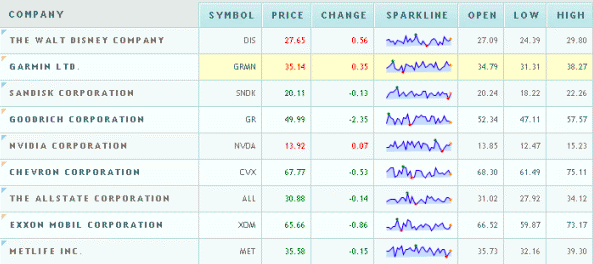
\includegraphics[width=1\linewidth]{images/stock-ticker.png}


Figura 1 — Uma aplicação de valores de Mercado em JavaScript

\textbf{Nota}: O \emph{feed} no Tópico do Mercado produz muitas atualizações de preço por segundo, então usar \emph{Polling} com um segundo de intervalo é mais prudente do que \emph{Long-Polling}, pois ele resultaria em uma série de \emph{Polls} contínuos. O \emph{Polling} controla de forma efetiva a vinda de atualizações.

% It all looks great, but a look under the hood reveals there are some serious issues with this application. For example, in Mozilla Firefox with Firebug (a Firefox add-on that allows you to debug web pages and monitor the time it takes to load pages and execute scripts), you can see that GET requests hammer the server at one-second intervals. Turning on Live HTTP Headers (another Firefox add-on that shows live HTTP header traffic) reveals the shocking amount of header overhead that is associated with each request. The following two examples show the HTTP header data for just a single request and response.
Tudo parece certo, mas ao se olhar o funcionamento, é revelado que há problemas sérios com essa aplicação. Por exemplo, com o \emph{Firebug}, você consegue ver que a requisição \code{GET} martela o Servidor em invervalos de 1 segundo. Ativando o \emph{Live HTTP Headers}, é revelado o enorme \emph{overhead} causado por cabeçalhos associados a cada requisição. Os dois próximos exemplos mostram o cabeçalho HTTP para somente uma requisição e uma resposta.

\textbf{Exemplo 1 — cabeçalho de requisição HTTP:}
\begin{lstlisting}
 GET /PollingStock//PollingStock HTTP/1.1
 Host: localhost:8080
 User-Agent: Mozilla/5.0 (Windows; U; Windows NT 5.1; en-US; rv:1.9.1.5)
 Gecko/20091102 Firefox/3.5.5
 Accept: text/html,application/xhtml+xml,application/xml;q=0.9,*/*;q=0.8
 Accept-Language: en-us
 Accept-Encoding: gzip,deflate
 Accept-Charset: ISO-8859-1,utf-8;q=0.7,*;q=0.7
 Keep-Alive: 300
 Connection: keep-alive
 Referer: http://www.example.com/PollingStock/
 Cookie: showInheritedConstant=false;
 showInheritedProtectedConstant=false;
 showInheritedProperty=false;
 showInheritedProtectedProperty=false;
 showInheritedMethod=false;
 showInheritedProtectedMethod=false;
 showInheritedEvent=false;
 showInheritedStyle=false;
 showInheritedEffect=false
\end{lstlisting}

\textbf{Exemplo 2 — cabeçalho de resposta HTTP}
\begin{lstlisting}
HTTP/1.x 200 OK
X-Powered-By: Servlet/2.5
Server: Sun Java System Application Server 9.1_02
Content-Type: text/html;charset=UTF-8
Content-Length: 21
Date: Sat, 07 Nov 2009 00:32:46 GMT
\end{lstlisting}

Só por diversão, eu contei todos os caracteres. O total de \emph{overhead} de informação na requisição e resposta HTTP é de 871 bytes, sem incuir nenhum dado! Claro, esse é somente um exemplo e você pode ter menos de 871 bytes de cabeçalho, mas eu também vi casos onde ele ultrapassava 2000 bytes. Nessa aplicação de exemplo, uma mensagem típica do Tópico de Mercado contém em torno de 20 caracteres. Como você pode ver, ela é efetivamente afogada pelo excesso de informação do cabeçalho, que nem é necessário no final das contas!

Então, o que acontece quando você dá \emph{deploy} nessa aplicação para um grande número de usuários? Vamos observar o tráfego de dados somente dos dados do cabeçalho HTTP de requisição e resposta associados a essa aplicação de \emph{Polling} em três casos diferentes.

\begin{itemize}
    \item \textbf{Caso de uso A}: 1,000 clientes fazendo \emph{Polling} a cada segundo: tráfego de dados é (871 x 1,000) = 871,000 bytes = 6,968,000 bits por segundo. (6.6 Mbps)
    \item \textbf{Caso de uso B}: 10,000 clientes fazendo \emph{Polling} a cada segundo: tráfego de dados é (871 x 10,000) = 8,710,000 bytes = 69,680,000 bits por segundo. (66 Mbps)
    \item \textbf{Caso de uso C}: 100,000 clientes fazendo \emph{Polling} a cada segundo: tráfego de dados é (871 x 100,000) = 87,100,000 bytes = 696,800,000 bits por segundo. (665 Mbps)
\end{itemize}

Essa é uma quatidade enorme de tráfego de dados desnecessários! Imagina só se fosse possível transferir a informação necessária. Então, com HTML5 Web Sockets você pode! Eu reconstrui a aplicação usando WebSockets, adicionando um manipulador de evento para que a página Web possa assincronamente ouvir por mensagens do \emph{Message Broker} de atualizações do preço do Mercado. Cada uma dessas mensagens é um WebSocket frame que possui só 2 bytes de overhead (ao invés de 871)! Veja como isso afeta o tráfego de dados de overhead naqueles três casos.

\begin{itemize}
    \item \textbf{Caso de uso A}: 1,000 clientes recebem 1 mensagem por segundo: Tráfego de dados é (2 x 1,000) = 2,000 bytes = 16,000 bits por segundo (0.015 Mbps)
    \item \textbf{Caso de uso B}: 10,000 clientes recebem 1 mensagem por segundo: Tráfego de dados é (2 x 10,000) = 20,000 bytes = 160,000 bits por segundo (0.153 Mbps)
    \item \textbf{Caso de uso C}: 100,000 clientes recebem 1 mensagem por segundo: Tráfego de dados é (2 x 100,000) = 200,000 bytes = 1,600,000 bits por segundo (1.526 Mbps)
\end{itemize}

Como você pode ver na figura abaixo, WebSocket provê uma redução dramática no tráfego de dados desnecessários em relação ao método de \emph{Polling}.

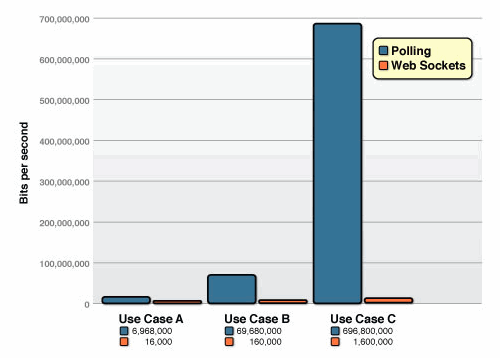
\includegraphics[width=1\linewidth]{images/comp.png}

Figura 2 — Comparação de \emph{overhead} entre aplicações de \emph{Polling} e \emph{WebSocket}.

E em relação à redução na latência? Veja a figura abaixo. Na metade de cima, você consegue a latência do método de \emph{Polling}. Se assumirmos, nesse exemplo, que é necessário 50 milissegundos para uma mensagem chegue do servidor ao \emph{browser}, então a aplicação de \emph{Polling} introduz muita latência extra, porque cada nova requisição precisa ser enviada ao servidor quando a resposta está completa. Essa nova requisição requer outros 50 milissegundos, e, durante esse tempo, o servidor não consegue mandar qualquer outra mensagem ao browser, resultando em um consumo de memória adicional ao servidor.

Na metade de baixo da figura, você vê a redução na latência proporcionada pelo uso de WebSocket. Uma vez que a conexão é promovida a WebSocket, as mensagens podem fluir do servidor ao browser no momento em que surgem. Ainda leva 50 milissegundos para as mensagens atravessarem do servidor ao cliente, mas a conexão WebSocket permanece aberta para que não haja necessidade de enviar outra requisição ao servidor.


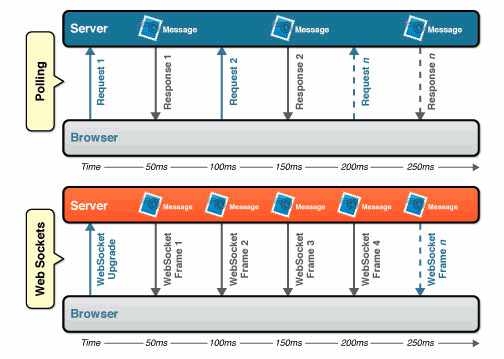
\includegraphics[width=1\linewidth]{images/latency.png}
Figura 3 — Comparação de latências entre \emph{Polling} e \emph{WebSocket}.
\end{quotation}




%----------------------------------------------------
\newpage
\paragraph{Em conclusão}

WebSocket é a solução ideal para problemas apresentados anteriormente. É um protocolo feito para a real comunicação plenamente bilateral e obtém isso com o menor gasto de recursos possível. Com ele, a criação de aplicações Web se torna muito mais viável e popular.

Mas existe um problema nesse meio de desenvolvimento Web, que é o fato de que a todo momento a infraestrutura é alterada. Novos protocolos são criados, outros são atualizados, antigos deixam de funcionar corretamente. Esse é um problema inerente ao meio e que afeta a todos.

Para ilustrar esse fato, vamos tomar como exemplo o protocolo \emph{SPDY} (pronunciado “speedy"), desenvolvido principalmente pela Google. \footnote{Ele não é um protocolo padrão, porém é bastante promissor e está sendo utilizado para o desenvolvimento do protocolo HTTP 2.0.}

Em linhas gerais, esse protocolo busca velocidade e se baseia no fato de que, se uma conexão é estabelecida com o servidor e o cliente começa a enviar muitas requisições HTTP, essas requisições vão incluir informações repetidas, comuns àquela sessão. Ele define então que, ao invés de enviar essas informações desnecessárias repetidamente durante a sessão, o servidor passa a salvar em um dicionário os usuários conectados e utilizar essas informações salvas. Por conta disso, fazer requisições passa a ser mais rápido e consumir menos recursos. \footnote{Note a semelhança com WebSockets.}

Também para aumentar a velocidade, o \emph{SPDY} multiplexa requisições para permitir que sejam feitas em paralelo. Atualmente no protocolo HTTP as requisições são todas feitas em série. O problema aparece nesse momento, pois o WebSocket esperava ter um socket TCP dedicado e agora passa a funcionar em cima de uma camada de conexão \emph{SPDY} multiplexada.

O WebSocket (assim como outros protocolos e ferramentas) necessita de  atualizações de tempos em tempos, por situações imprevisíveis como essa. Essa mudança constante aumenta o nível de dificuldade para o desenvolvedor estar sempre atualizado com seus detalhes de implementação.

Uma das maneiras de se contornar essa dificuldade é utillizar outras APIs que cuidam desses detalhes internamente.


\subsubsection{Socket.io}

Por fim, foi criado o Socket.io, uma API de WebSocket para JavaScript. Ela cuida de todos os detalhes de funcionamento do protocolo internamente, deixando uma interface simples ao usuário. Assim, mudanças no funcionamento do protocolo não chegam ao desenvolvedor.

Para uma conexão ser estabelecida, tanto o cliente quanto o servidor precisam estar executando Socket.io. Sua implementação tenta primeiramente fazer a conexão usando WebSocket, mas se o servidor não suporta esse protocolo, ele recua (faz \emph{fallback}) para outras tecnologias, como \emph{AJAX long-polling}, \emph{AJAX multipart streaming}, \emph{IFrame}, \emph{JSONP polling}, entre outros (todos utilizando a mesma interface). Esse \emph{fallback} permite à API abranger uma quantidade muito maior de servidores, reduzindo possíveis problemas numa implementação em larga escala.

Além da implementação básica do protocolo WebSocket, ele também adiciona outras funcionalidades importantes para o desenvolvimento de uma aplicação mais robusta:

\begin{itemize}

\item \textbf{A possibilidade de criação arbritrária de eventos}. Além dos eventos padrões \emph{'connect'}, \emph{'message'} e \emph{'disconnect'}, o desenvolvedor pode criar quaisquer outros eventos que achar necessário.

Essa criação de eventos funciona da seguinte forma: o processo emissor manda a mensagem e o nome do evento que está sendo enviado. O processo receptor define o evento que vai ouvir e a subrotina que vai ser executada na ocorrência desse evento. Se o evento lançado for ouvido pelo receptor, o \emph{callback} é chamado.

Com WebSocket, o desenvolvedor fica preso aos quatro eventos pré definidos: \emph{'onopen'}, \emph{'onclose'}, \emph{'onmessage'} e \emph{'onerror'}. Internamente, os quatro são eventos de mensagem, disparados em momentos e situações específicas. O que o Socket.io faz é dar a liberdade de definir quaisquer eventos desejados.

\item \textbf{A possibilidade de conectar múltiplos sockets em uma mesma porta}. Internamente, ele faz uma multiplexação das várias conexões abertas em uma mesma porta, mas os processos entendem que tem um socket dedicado a eles. Utilizando WebSockets, cada socket precisa de uma porta exclusiva para fazer a conexão.

A possibilidade de vários sockets em uma mesma aplicação permite uma modularização muito maior, pois não é necessário que um módulo saiba se tem uma conexão dedicada ou se está compartilhando com mais dezenas de outros sockets.

Um ponto negativo dessa definição de eventos é que o cabeçalho da mensagem é um pouco maior, pois o de WebSockets é reduzido ao extremo, mas esse tamanho ainda é ínfimo e o \emph{overhead} causado não se torna um problema.

\item \textbf{Definição de \emph{namespaces}}. Dada a existência de múltipos sockets, é possível organizá-los em \emph{namespaces}. Cada \emph{namespace}
vai conter um conjunto de sockets conectados, e eventos emitidos a um \emph{namespace} serão enviados somente à esse conjunto.

Por padrão, caso nenhum \emph{namespace} seja definido, todos os sockets são conectados ao \emph{namespace} \emph{'/'}. Assim, esse funcionamento fica invisível ao desenvolvedor que não os está utilizando.

\item \textbf{Definição de \emph{rooms}}. \emph{Rooms} são um segundo nível de organização, definidos dentro de \emph{namespaces}. Um socket pode entrar e sair de \emph{rooms} com funções \code{join} e \code{leave}. Cada socket pode definir uma \emph{room} específica na hora de emitir um evento, da forma:

\code{io.to('some room').emit('some event')}

\end{itemize}

É fácil notar a preocupação com organização dessas funcionalidades. Com o protocolo WebSocket puro, é inviável fazer uma aplicação que faz o uso de múltiplos sockets com execuções distintas, mas que interagem entre si. Um dos propósitos da criação de Socket.io foi aumentar o grau de liberdade do desenvolvedor e tornar esse tipo de aplicação muito simples de ser desenvolvida.

\newpage

% \section{Evolução do Projeto}

% Esse projeto utiliza várias tecnologias que eu nunca tive contato.


% Inicialmente a ideia inicial do TCC era usar um Arduino e um conjunto de sensores para coletar dados do meio e mandar de maneira síncrona para um servidor. O servidor então usaria esses dados para fazer algum controle. Numa primeira discussão com o orientador, a ideia foi rapidamente descartada, pelos seguintes motivos:

% Os sensores dele normalmente são imprecisos;
% A montagem de um dispositivo como o idealizado seria desnecessariamente custosa e muito propensa a erros;
% Sem uma montagem muito bem executada, o dispositivo ficaria muito frágil;
% É possível conseguir muitas leituras de sensores utilizando um smartphone.


% Com os argumentos apresentados, a decisão foi criar um aplicativo para Android com o mesmo propósito. Todos os argumentos apresentados são resolvidos com essa solução. A implementação é extremamente mais simples; os sensores são muito mais precisos; a estrutura física já está pronta e é um objeto que já está presente em todo o mundo (o produto final atinge grande parte da população); e, por fim, é muito viável a adição ou remoção de funcionalidades, além de muito mais suporte para a plataforma.


% Uma vez que a decisão de utilizar um smartphone, foi necessário saber como implementar um aplicativo que tenha acesso aos sensores.
% A primeira ideia foi utilizar serviço MIT App Inventor.

% \section{Tecnologias citadas}

% \subsection{MIT App Inventor}

% É um serviço disponibilizado pelo MIT para a criação de aplicativos. Ele é extremamente didático e inclusivo, sua interface não é dada por linhas de código, e sim por blocos lógicos que se encaixam e formam um algoritmo (na prática, é bastante ruim não poder escrever linhas de código livremente). Sua API possui interface para o uso de sensores, além de outras funcionalidades que não foram exploradas neste TCC, como acesso à ferramenta de reconhecimento de voz e ferramentas sociais, como email, mensagem e Twitter. O serviço é bom, porém possui várias restrições, então é difícil de ser usado.


% Com certa dificuldade um primeiro aplicativo de teste foi feito, para pegar valores do giroscópio. O próximo passo seria criar um servidor e estabelecer uma conexão entre ambos, porém as opções de conectividade do App Inventor também são muito restritas, então, dada a dificuldade prevista, eu achei melhor deixar essa plataforma de lado no momento e procurar outras alternativas para a criação de um app.


% \subsection{Kivy}

% É um framework Open Source de Python. Seu objetivo é o desenvolvimento rápido de aplicações multiplataforma que fazem o uso de interfaces inovadoras, como telas com Multitouch e sensores de movimento. Sua API, por exemplo, lida com eventos de mouse, teclado e toques de tela. Ele também possui um foco na criação de apps com NUI (Natural User Interface).
%   NUI é uma metodologia de interface cuja proposta é ser invisível ao usuário, e apresentar uma experiência natural e intuitiva. Seu principal foco é evitar grandes barreiras durante o aprendizado. Através de decisões de design, o usuário tem um entendimento do software sem grandes dificuldades, à medida que a complexidade da interação aumenta.

% [TODO] Para exemplificar a facilidade de desenvolvimento de lógica e de uma interface gráfica, abaixo tem o código para se criar um jogo de Pong.



% \section{Casos de Uso}


% TODO Apendice: falar do SPDY (protocolo tipo http)

\newpage
\section{Conclusão}

O Projeto propõe um ambiente Web de comunicação entre smartphones executando o aplicativo desenvolvido e a página Web que recebe dados para alterar seu funcionamento, através de um Servidor que permite a comunicação da maneira eficiente e viável.

Os dois maiores desafios nessa proposta eram:

\begin{itemize}
    \item Encontrar uma forma de comunicação que atendesse à todas as necessidades dessa arquitetura;
    \item Desenvolver essa arquitetura para servir de base para projetos de maior porte.
\end{itemize}

O primeiro item é resolvido com a utilização do \textbf{Socket.io}. Ele é a ferramenta ideal para lidar com a comunicação entre os clientes e o servidor, tendo em vista todos os requerimentos apresentados. Além de ideal, sua interface também é muito simples de ser usada e é um aspecto positivo para o segundo item.

Para o segundo item, foi necessário encontrar as ferramentas corretas.

O \textbf{Apache Cordova} permite o desenvolvimento de aplicativos para Android (além de outras plataformas) igual ao desenvolvimento Web. Este ponto facilita na hora de se desenvolver um aplicativo em conjunto com uma aplicação Web.

\textbf{Node.js} e \textbf{Express} tornam a criação de um servidor muito simples e direta, com o funcionamento desejado para a comunicação entre os clientes.

A aplicação Web está menos definida, mas no caso de uso apresentado, \textbf{THREE.js} permite a criação 3D de forma direta, abstraindo detalhes de implementação de bibliotecas 3D de baixo nível.

Todas essas ferramentas funcionam bem entre si e permitem o desenvolvimento rápido e direto de projetos maiores e escaláveis. Por fim, é concluido que o ambiente Web funciona bem e o Projeto foi bem sucedido na proposta apresentada.


\newpage

\begin{thebibliography}{50}
\bibitem{websocket_quantum}
HTML5 WebSocket - A Quantum Leap in Scalability for the Web,
\\\texttt{\url{https://www.websocket.org/quantum.html}}

Acessado em: 20/11/16


\bibitem{websocket_prot}
RFC 6455 - The WebSocket Protocol,
\\\texttt{\url{https://tools.ietf.org/html/rfc6455}}

Acessado em: 20/11/16


\bibitem{socket_yt}
Computer Networks 1-4: Sockets,
\\\texttt{\url{https://www.youtube.com/watch?v=zWqLYby99EU}}

Acessado em: 20/11/16


\bibitem{socket_oracle}
What Is a Socket?,
\\\texttt{\url{https://docs.oracle.com/javase/tutorial/networking/sockets/definition.html}}

Acessado em: 20/11/16


\bibitem{socket_websocket}
node.js - Differences between socket.io and websockets - Stack Overflow,
\\\texttt{\url{http://stackoverflow.com/questions/10112178/differences-between-socket-io-and-websockets}}

Acessado em: 20/11/16


\bibitem{polling_stackoverflow}
 - What are Long-Polling, Websockets, Server-Sent Events (SSE) and Comet? - Stack Overflow,
\\\texttt{\url{http://stackoverflow.com/questions/11077857/what-are-long-polling-websockets-server-sent-events-sse-and-comet}}

Acessado em: 20/11/16


\bibitem{long_polling_timeout_stackoverflow}
javascript - HTTP Long Polling - Timeout best practice - Stack Overflow,
\\\texttt{\url{http://stackoverflow.com/questions/37391096/http-long-polling-timeout-best-practice}}

Acessado em: 20/11/16


\bibitem{threejs_guide}
The Beginners Guide to three.js - Treehouse Blog,
\\\texttt{\url{http://blog.teamtreehouse.com/the-beginners-guide-to-three-js}}

Acessado em: 20/11/16


\bibitem{socketio}
Socket.IO,
\\\texttt{\url{http://socket.io/}}

Acessado em: 20/11/16


\bibitem{cordova}
Apache Cordova,
\\\texttt{\url{https://cordova.apache.org/}}

Acessado em: 20/11/16


\bibitem{sockerio_cordova}
Socket.IO  —  Socket.IO with Apache Cordova,
\\\texttt{\url{http://socket.io/socket-io-with-apache-cordova/}}

Acessado em: 20/11/16


\bibitem{cordova_tutpoint}
Cordova Tutorial,
\\\texttt{\url{http://www.tutorialspoint.com/cordova/}}

Acessado em: 20/11/16


\bibitem{three_scene}
three.js / documentation - Creating a scene,
\\\texttt{\url{https://threejs.org/docs/index.html\#Manual/Introduction/Creating_a_scene}}

Acessado em: 20/11/16


\bibitem{websocket_socketio}
WebSocket and Socket.IO,
\\\texttt{\url{https://davidwalsh.name/websocket}}

Acessado em: 20/11/16


\bibitem{webgl_wiki}
WebGL,
\\\texttt{\url{https://en.wikipedia.org/wiki/WebGL}}

Acessado em: 20/11/16


\bibitem{threejs_wiki}
Three.js,
\\\texttt{\url{https://en.wikipedia.org/wiki/Three.js}}

Acessado em: 20/11/16


\bibitem{node_yt}
What is Node.js Exactly? - a beginners introduction to Nodejs,
\\\texttt{\url{https://www.youtube.com/watch?v=pU9Q6oiQNd0}}

Acessado em: 20/11/16


\bibitem{nodejs}
Node.js,
\\\texttt{\url{https://nodejs.org/en/}}

Acessado em: 20/11/16


\bibitem{nodejs_tutorial}
Node.js Introduction,
\\\texttt{\url{https://www.tutorialspoint.com//nodejs/nodejs_introduction.htm}}

Acessado em: 20/11/16


\bibitem{express_tutorial}
ExpressJS Tutorial,
\\\texttt{\url{http://www.tutorialspoint.com/expressjs/index.htm}}

Acessado em: 20/11/16


\bibitem{http_easy}
HTTP Made Really Easy,
\\\texttt{\url{https://www.jmarshall.com/easy/http/}}

Acessado em: 20/11/16


\bibitem{ajax_tutorial}
What Is Ajax?,
\\\texttt{\url{https://www.tutorialspoint.com/ajax/what_is_ajax.htm}}

Acessado em: 20/11/16


\bibitem{websocket_about}
About HTML5 WebSocket,
\\\texttt{\url{https://www.websocket.org/aboutwebsocket.html}}

Acessado em: 20/11/16


\bibitem{spdy_wiki}
SPDY,
\\\texttt{\url{https://pt.wikipedia.org/wiki/SPDY}}

Acessado em: 20/11/16


\bibitem{how_web-page}
How Web Pages Work,
\\\texttt{\url{http://computer.howstuffworks.com/web-page.htm}}

Acessado em: 04/02/17



\end{thebibliography}


\end{document}
